% **************************************************************
% Hi! Edit this file for your presentation!
% **************************************************************

% ==================///==================///==================///
% ==================/// LATEX'S STUFF
% ==================///==================///==================///

\documentclass{beamer}
\usepackage{amsfonts,amsmath,oldgerm}
% Attiva i bordi arrotondati e l'ombra per i blocchi
\setbeamertemplate{blocks}[rounded][shadow=true]
\usepackage{booktabs}
% Imposta i colori (modifica "blue" con il colore del tuo tema)
\setbeamercolor{block title}{bg=blue!70!black, fg=white}
\setbeamercolor{block body}{bg=blue!10, fg=black}
\definecolor{blustatale}{RGB}{7,27,80} % Blu ufficiale Unimi
\usepackage{tcolorbox}
\usetheme{_statale}
\usefonttheme[onlymath]{serif}
\usepackage{tikz}
\newcommand{\testcolor}[1]{\colorbox{#1}{\textcolor{#1}{test}}~\texttt{#1}}
\newcommand{\hrefcol}[2]{\textcolor{cyan}{\href{#1}{#2}}}
\titlebackground*{assets/background}
\date{October 5, 2026}

% ==================///==================///==================///
% ==================/// SPLASH PAGE
% ==================///==================///==================///

\title{Comparative Study of Homogeneous and Sampling Electromagnetic Calorimeters}
\subtitle{A Geant4 and ROOT Analysis of Shower Containment, Passive Material Effects, and Sampling Fluctuations in $PbWO_4$ and $LAr/Pb$}
%\course{Master's Degree in Physics}
\author{\href{mailto:nicolo.favagrossa@studenti.unimi.it}{Nicolò Favagrossa}}
%\IDnumber{68405A}

% ==================///==================///==================///
% ==================/// START PRESENTATION
% ==================///==================///==================///

\begin{document}
\maketitle

\footlinecolor{maincolor}

% ==================///==================///==================///
% ==================/// BODY'S PRESENTATION
% ==================///==================///==================///

\begin{frame}{Introduction to the simulated calorimeters}
    \begin{table}
        \centering
        \renewcommand{\arraystretch}{1.5} % Aumenta la spaziatura verticale tra le righe per maggiore leggibilità
        \begin{tabular}{@{} p{0.22\textwidth} p{0.35\textwidth} p{0.35\textwidth} @{}}
            \toprule
            & \textbf{Homogeneous} (CMS) & \textbf{Sampling} (ATLAS) \\
            \midrule
            
            \textbf{Material} & 
            Lead Tungstate ($PbWO_4$) crystals & 
            Lead (Pb) absorber + Liquid Argon (LAr) active medium \\
            
            \textbf{Working Principle} & 
            A single medium acts simultaneously as both the full absorber and the active detector. & 
            Passive layers absorb the majority of energy, while active layers sample the shower. \\
            
            \textbf{Characteristics} & 
            Short $X_0$ ($\approx 0.89$ cm) results in a highly compact design with good energy resolution. & 
            Highly radiation-resistant design for optimal longitudinal segmentation. \\
            
            \bottomrule
        \end{tabular}
    \end{table}
\end{frame}

\begin{frame}{Electromagnetic shower containment in PbWO$_4$}
    \begin{columns}
        % Left Column: Theoretical framework
        \begin{column}{0.50\textwidth}
            Simulating 100 GeV electrons:
            \begin{itemize}
                \item Lead Tungstate ($\text{PbWO}_4$) is extremely dense, featuring a short radiation length ($X_0 \approx 0.89\,\text{cm}$).
                \item Standard electromagnetic calorimeter design requires approximately $25\,X_0$ to effectively contain the shower and its tail.
                \item The $98\%$ energy containment threshold to be reached at approximately $22\,\text{cm}$ of thickness.
            \end{itemize}
        \end{column}
        
        % Right Column: Simulation results
        \begin{column}{0.50\textwidth}
            \begin{figure}
                \centering
                % Replace 'plot.png' with the actual filename of your graph
                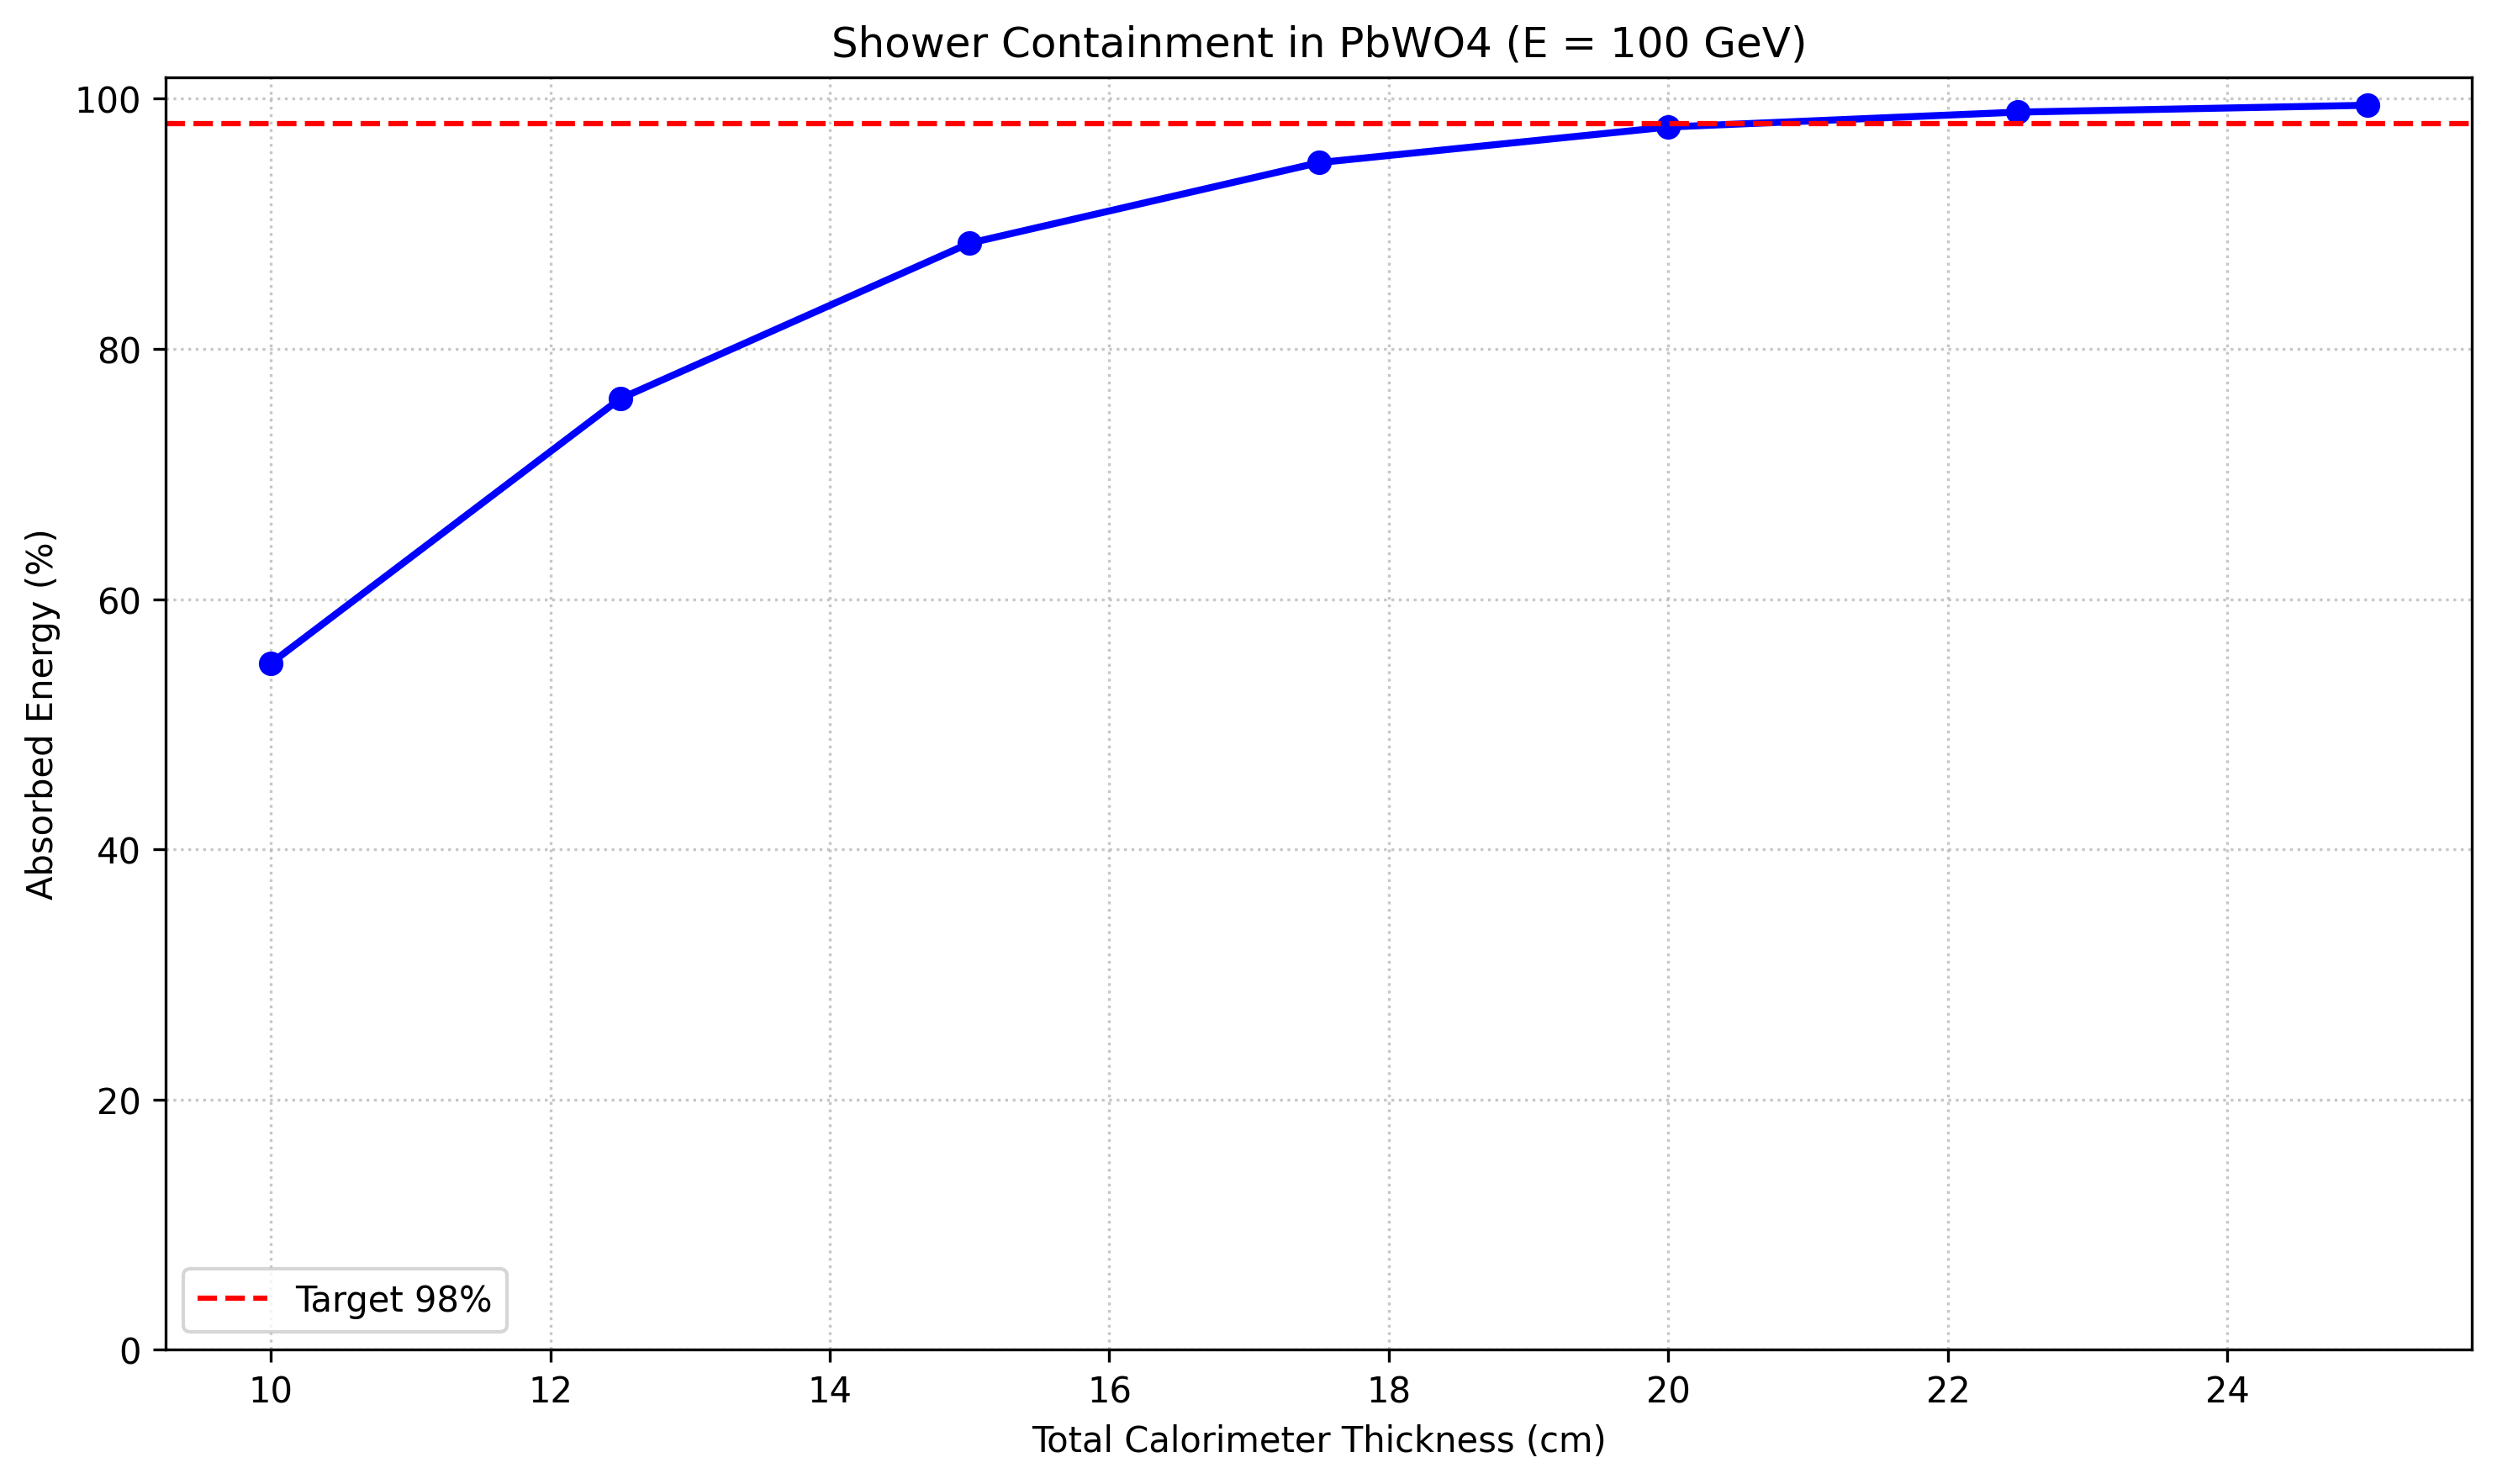
\includegraphics[width=\textwidth]{Immagini/risultati_contenimento.png} 
            \end{figure}
            
                The simulation confirms the expected longitudinal development.
        \end{column}
    \end{columns}
\end{frame}

\begin{frame}{Impact of longitudinal leakage on energy resolution}

    Incomplete longitudinal containment introduces severe statistical fluctuations in the measured energy. As the containment approaches $100\%$, leakage vanishes and the energy resolution $\sigma/\langle E \rangle$ drops, as demonstrated below for $10\,\text{GeV}$ $e^-$.
    
    
    \begin{columns}[c]
        % Colonna sinistra: Grafico
        \begin{column}{0.55\textwidth}
            \begin{figure}
                \centering
                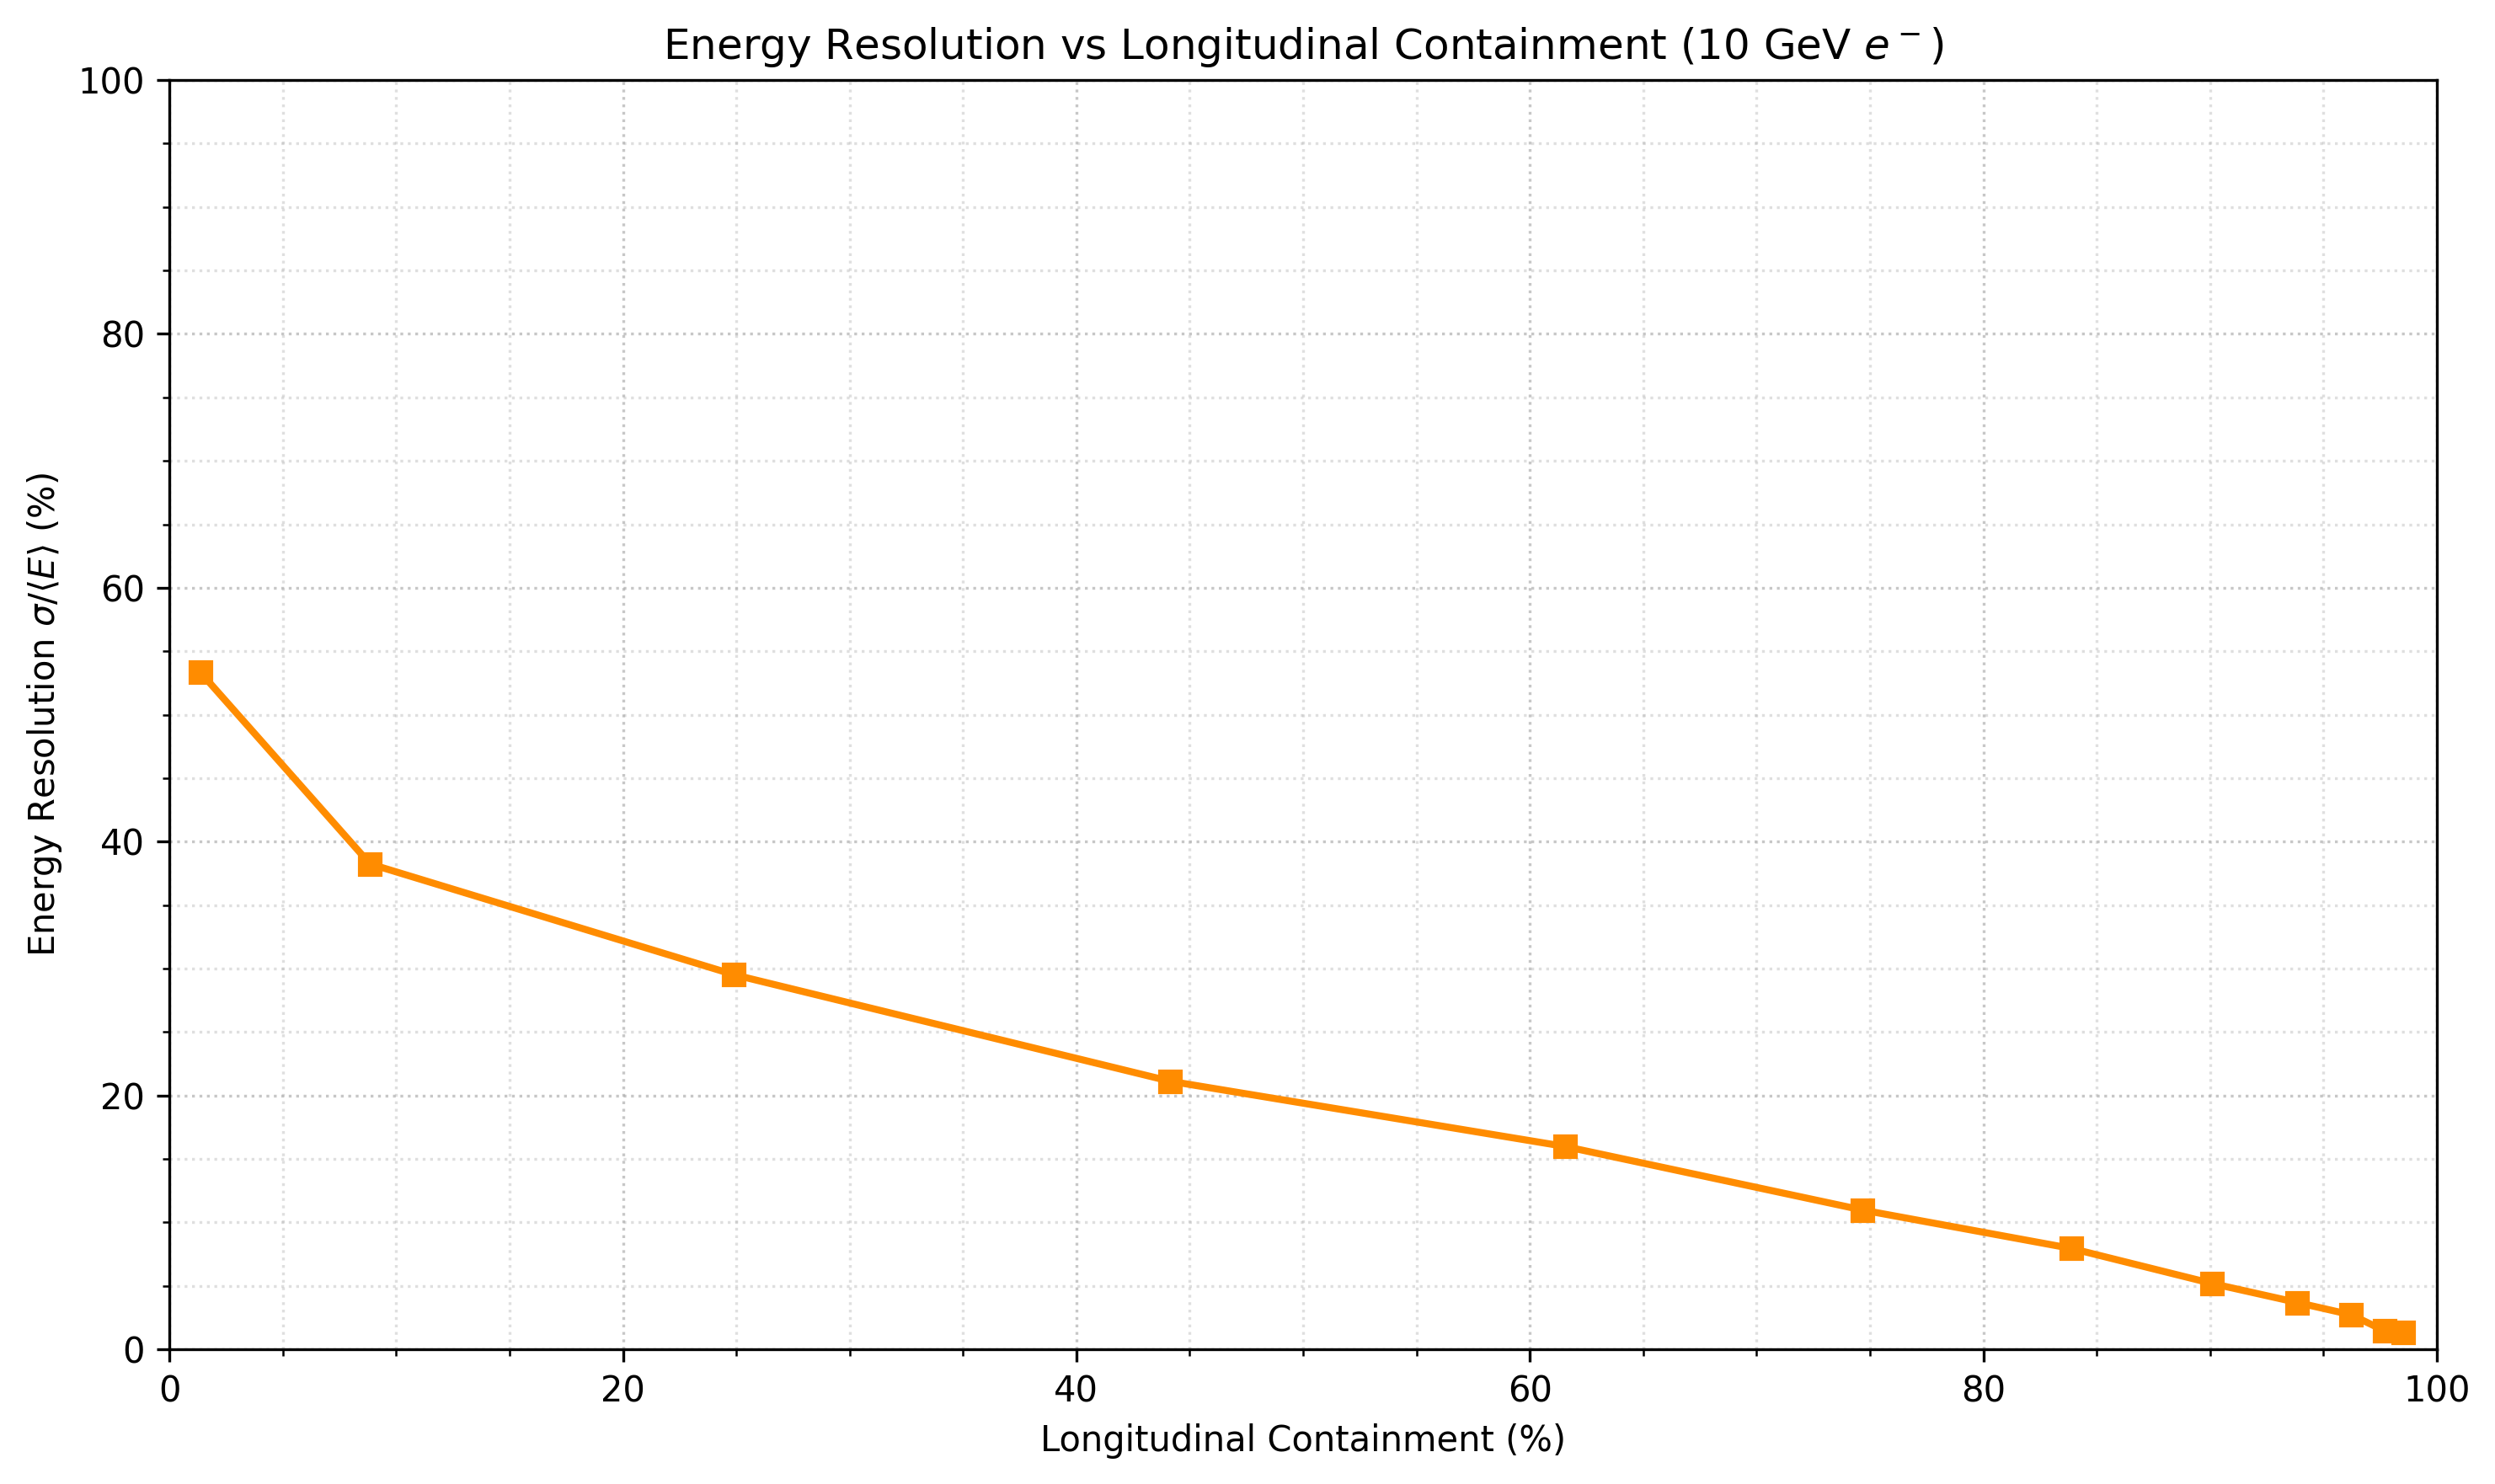
\includegraphics[width=\textwidth]{Immagini/risultati_risoluzione.png}
            \end{figure}
        \end{column}
        
        % Colonna destra: Tabella dati
        \begin{column}{0.45\textwidth}
            \centering
            \scriptsize % Font ridotto per far stare tutte le 12 righe
            \renewcommand{\arraystretch}{1.1} % Leggera spaziatura verticale
            \begin{tabular}{@{} cccc @{}}
                \toprule
                \textbf{Depth} & \textbf{Depth} & \textbf{Cont.} & \textbf{$\sigma/\langle E \rangle$} \\
                \textbf{[cm]} & \textbf{[$X_0$]} & \textbf{[\%]} & \textbf{[\%]} \\
                \midrule
                2.50  & 2.81  & 1.35  & 53.35 \\
                4.00  & 4.49  & 8.84  & 38.25 \\
                5.50  & 6.18  & 24.89 & 29.52 \\
                8.50  & 9.55  & 61.54 & 15.99 \\
                10.00 & 11.24 & 74.65 & 10.99 \\
                11.50 & 12.92 & 83.88 & 7.95  \\
                13.00 & 14.61 & 90.09 & 5.19  \\
                14.50 & 16.29 & 93.86 & 3.69  \\
                19.00 & 21.35 & 98.53 & 1.31  \\
                \bottomrule
            \end{tabular}
        \end{column}
    \end{columns}

\end{frame}

\begin{frame}{Effect of upstream dead material on resolution}

    The presence of inactive material (e.g., a tracker) in front of the calorimeter negatively impacts energy resolution. Simulating $10\,\text{GeV}$ $e^-$ traversing a Lead (Pb) layer from $0.1$ to $1.0\,\text{cm}$ demonstrates how unmeasured energy loss from early shower initiation causes a severe degradation in performance.
        \vspace{-0.3cm}
    \begin{columns}[c]
        % Colonna sinistra: Grafico
        \begin{column}{0.60\textwidth}
            \begin{figure}
                \centering
                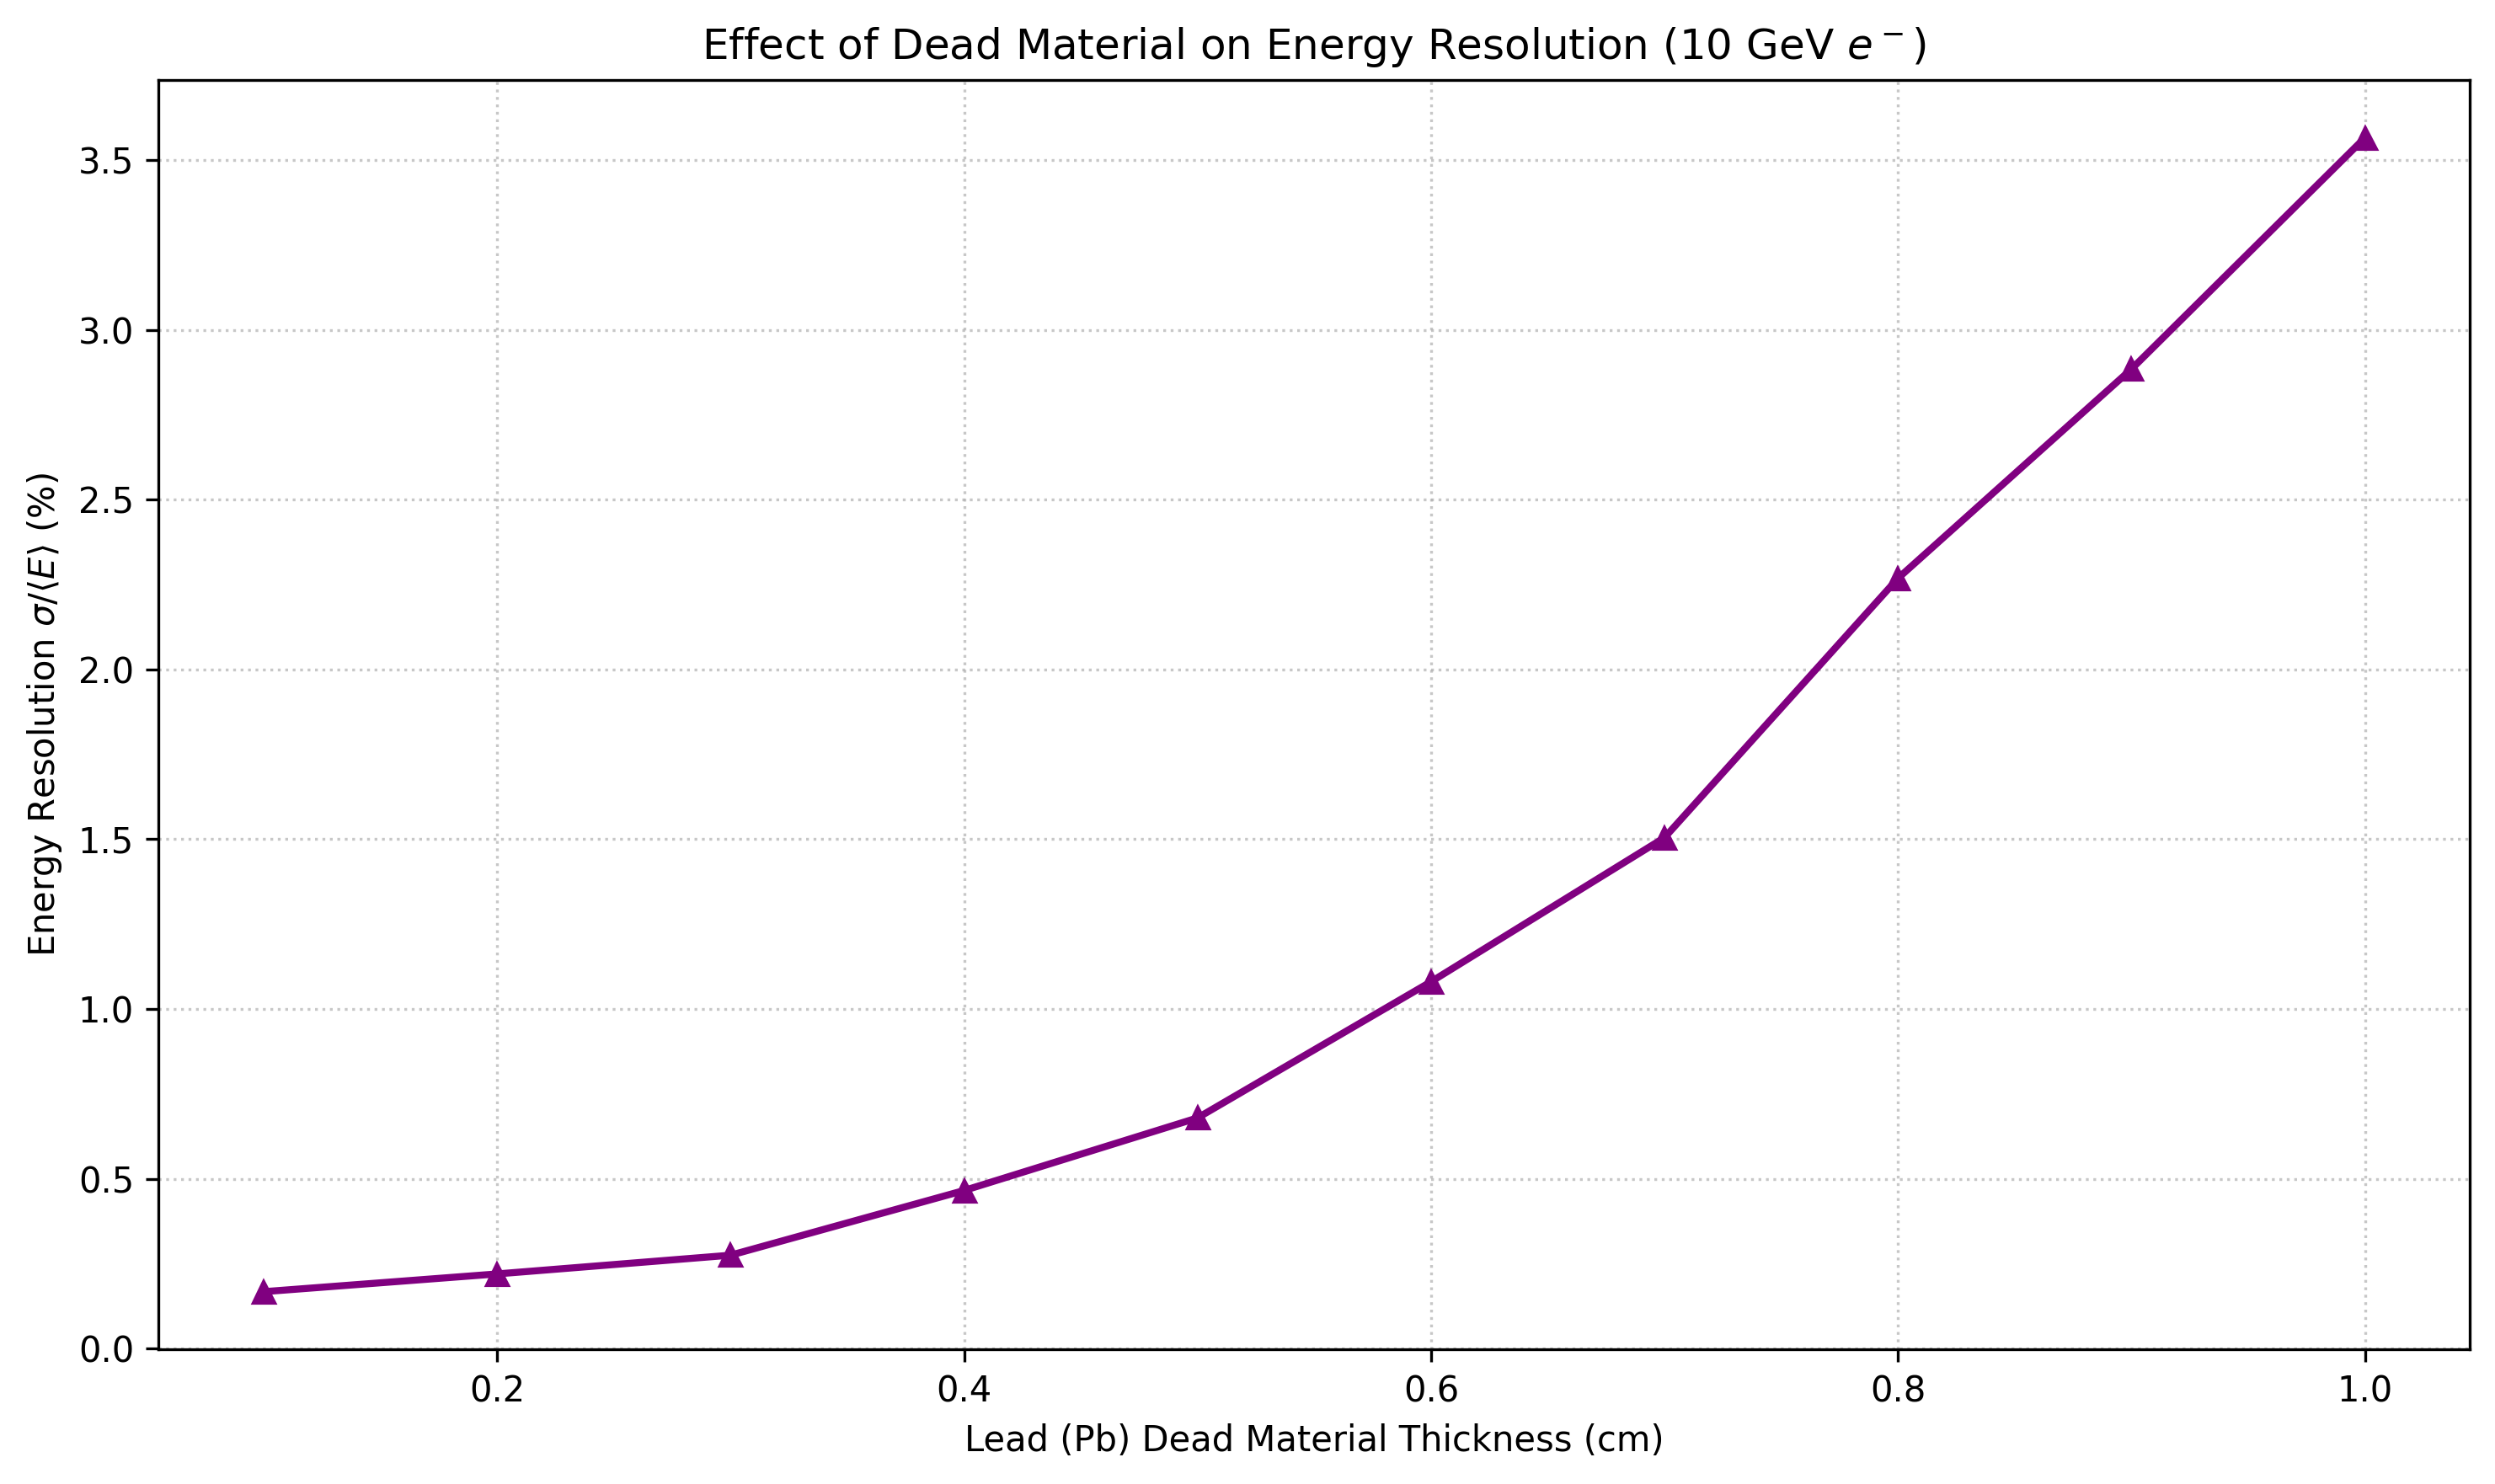
\includegraphics[width=0.9\textwidth]{Immagini/dead_material_resolution.png}
            \end{figure}
        \end{column}
        
        % Colonna destra: Tabella dati
        \begin{column}{0.40\textwidth}
            \centering
            \footnotesize % Font adeguato per 10 righe
            \renewcommand{\arraystretch}{1} % Migliora la leggibilità verticale
            \begin{tabular}{@{} cc @{}}
                \toprule
                \textbf{Pb Depth} & \textbf{$\sigma/\langle E \rangle$} \\
                \textbf{[cm]} & \textbf{[\%]} \\
                \midrule
                0.10 & 0.17 \\
                0.20 & 0.22 \\
                0.30 & 0.27 \\
                0.80 & 2.27 \\
                0.90 & 2.89 \\
                1.00 & 3.57 \\
                \bottomrule
            \end{tabular}
        \end{column}
    \end{columns}

\end{frame}

\begin{frame}{Optimal cell size: transverse containment}
    \begin{columns}[T] 
        
        % Left Column: Theory and Conclusion (35% width)
        \begin{column}{0.35\textwidth}
            
            The ideal cell size is dictated by the Molière radius ($R_M$), which encloses $\sim 87\%$ of the transverse shower energy.
            
            \vspace{0.3cm}
            \begin{itemize}
                \item $R_M(PbWO_4) = 2.2\,\text{cm}$
            \end{itemize}
            
            \vspace{0.3cm}
            Simulation reaches the $87\%$ target exactly at $R = 2.01\,\text{cm}$.
        \end{column}
        
        % Right Column: Only the graph (65% width)
        \begin{column}{0.65\textwidth}
            \begin{figure}
                \centering
                % Assicurati che il nome e il percorso del file siano corretti
                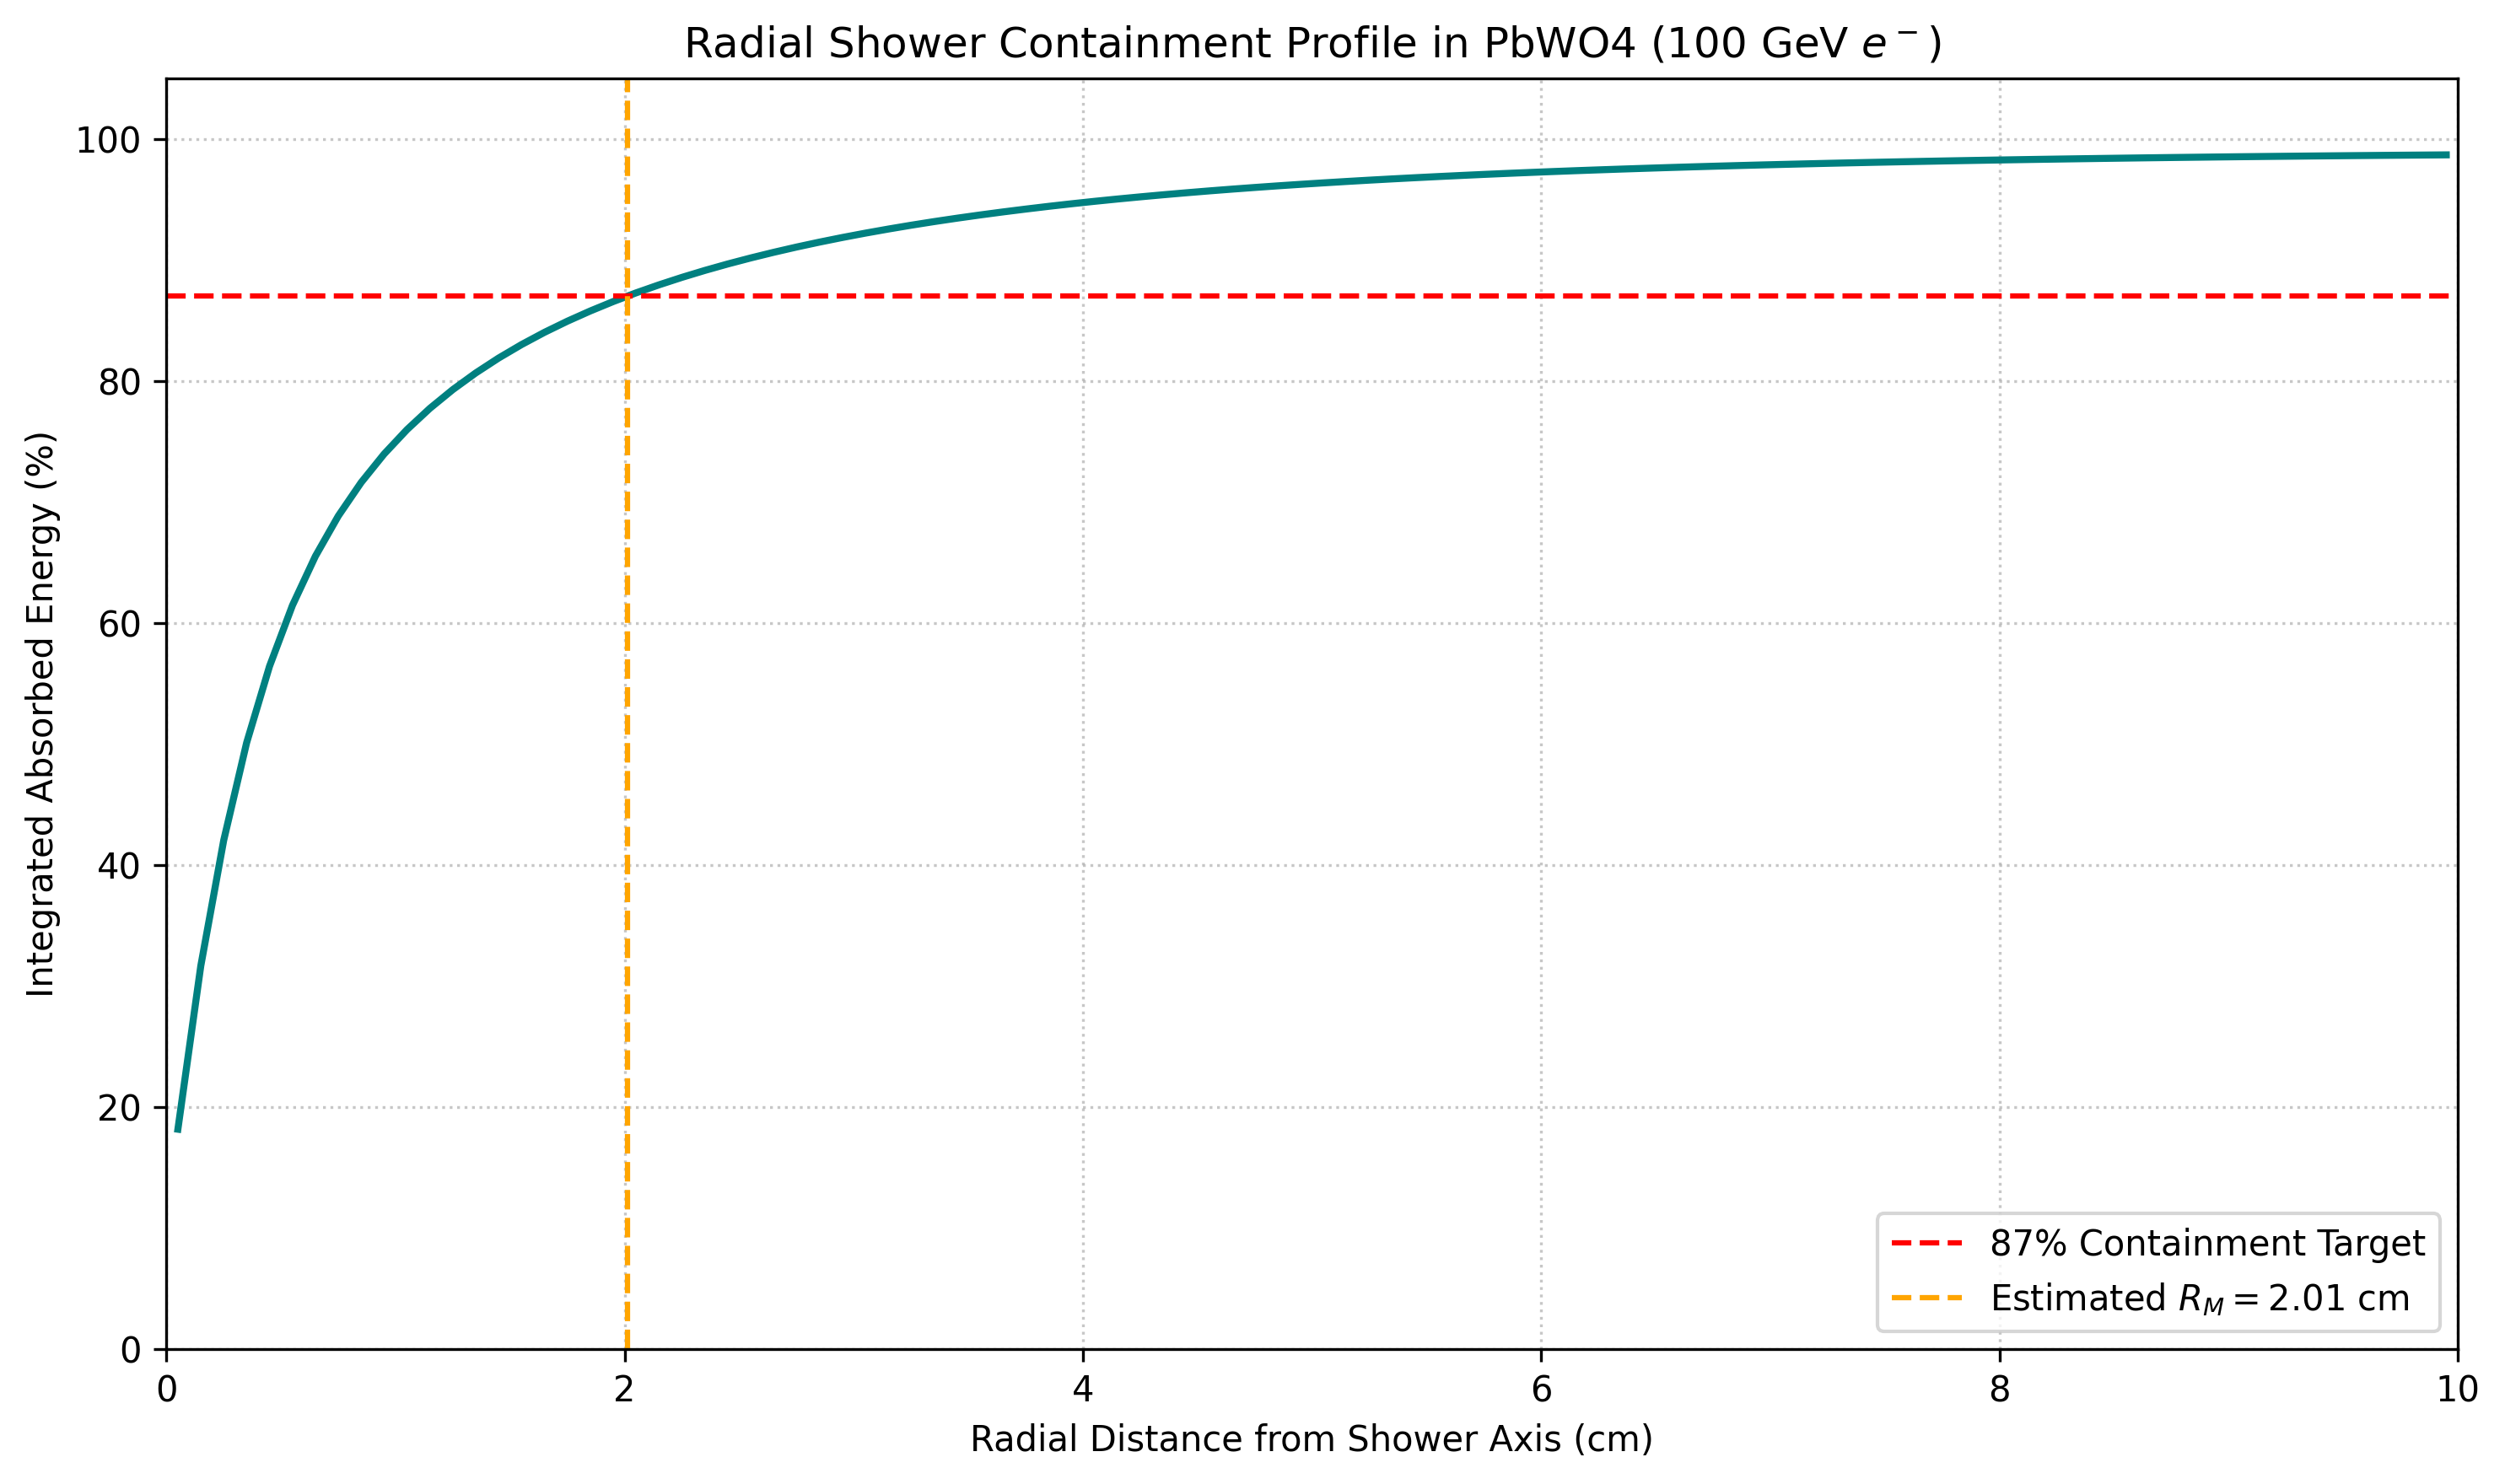
\includegraphics[width=\textwidth, keepaspectratio]{Immagini/radial_containment_moliere.png} 
            \end{figure}
        \end{column}
        
    \end{columns}
\end{frame}


%\begin{frame}{Energy Response: The Resolution Anomaly}
%
%    \begin{itemize}
%        \item Shower maximum ($t_{max}$) scales with $\ln(E)$.
%        \item At $20\text{--}100\,\text{GeV}$, shower tails escape the $25\,\text{cm}$ detector.
%        \item Fluctuations in leaked energy break the ideal $1/\sqrt{E}$ scaling.
%    \end{itemize}
%    
%    \vspace{-0.2cm}
%    \begin{figure}
%        \centering
%        % Sostituisci con il nome corretto del file
%        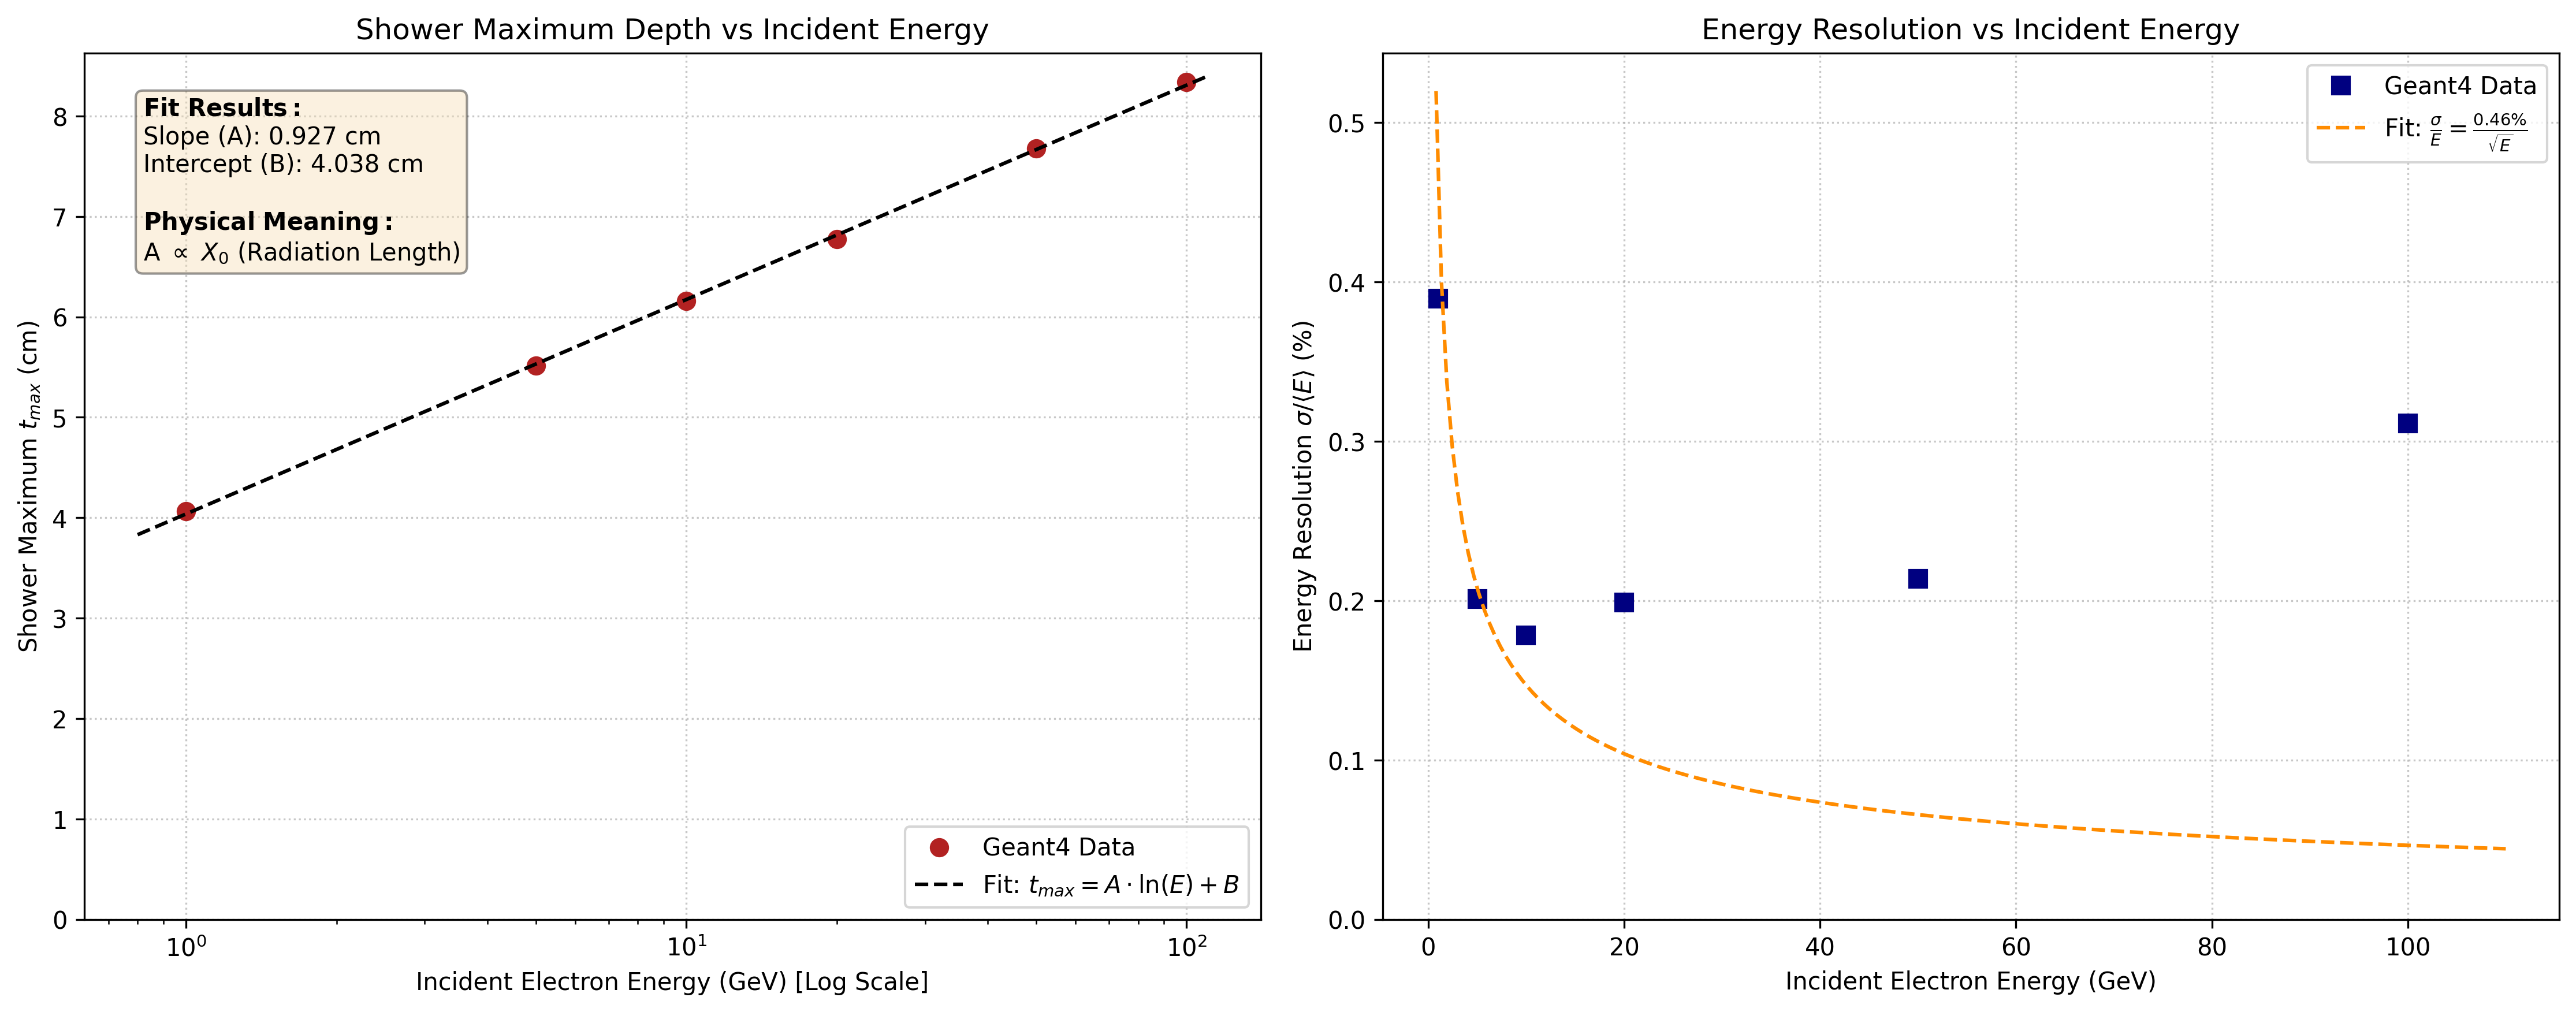
\includegraphics[width=0.9\textwidth, keepaspectratio]{Immagini/energy_response_analysis.png}
%    \end{figure}

%\end{frame}




%\begin{frame}{Energy Response: The Resolution Anomaly}
%
%    \small % Riduce leggermente il font per ospitare il nuovo concetto
%    \begin{itemize}
%        \setlength{\itemsep}{3pt} % Comprime leggermente lo spazio verticale tra i punti
%        
%        \item Shower maximum ($t_{max}$) scales with $\ln(E)$. Above $20\,\text{GeV}$, shower tails begin to escape the $25\,\text{cm}$ detector.
%        
%        \item Lacking photon production and collection inefficiencies, the simulated intrinsic stochastic term is artificially tiny ($\sim 0.46\%/\sqrt{E}$).
%        
%        \item Because this baseline intrinsic error is so small, even minor longitudinal leakage fluctuations severely dominate the resolution, breaking the $1/\sqrt{E}$ scaling (an effect usually masked in sampling calorimeters).
%    \end{itemize}
%    
%    \vspace{-0.2cm}
%    \begin{figure}
%        \centering
%        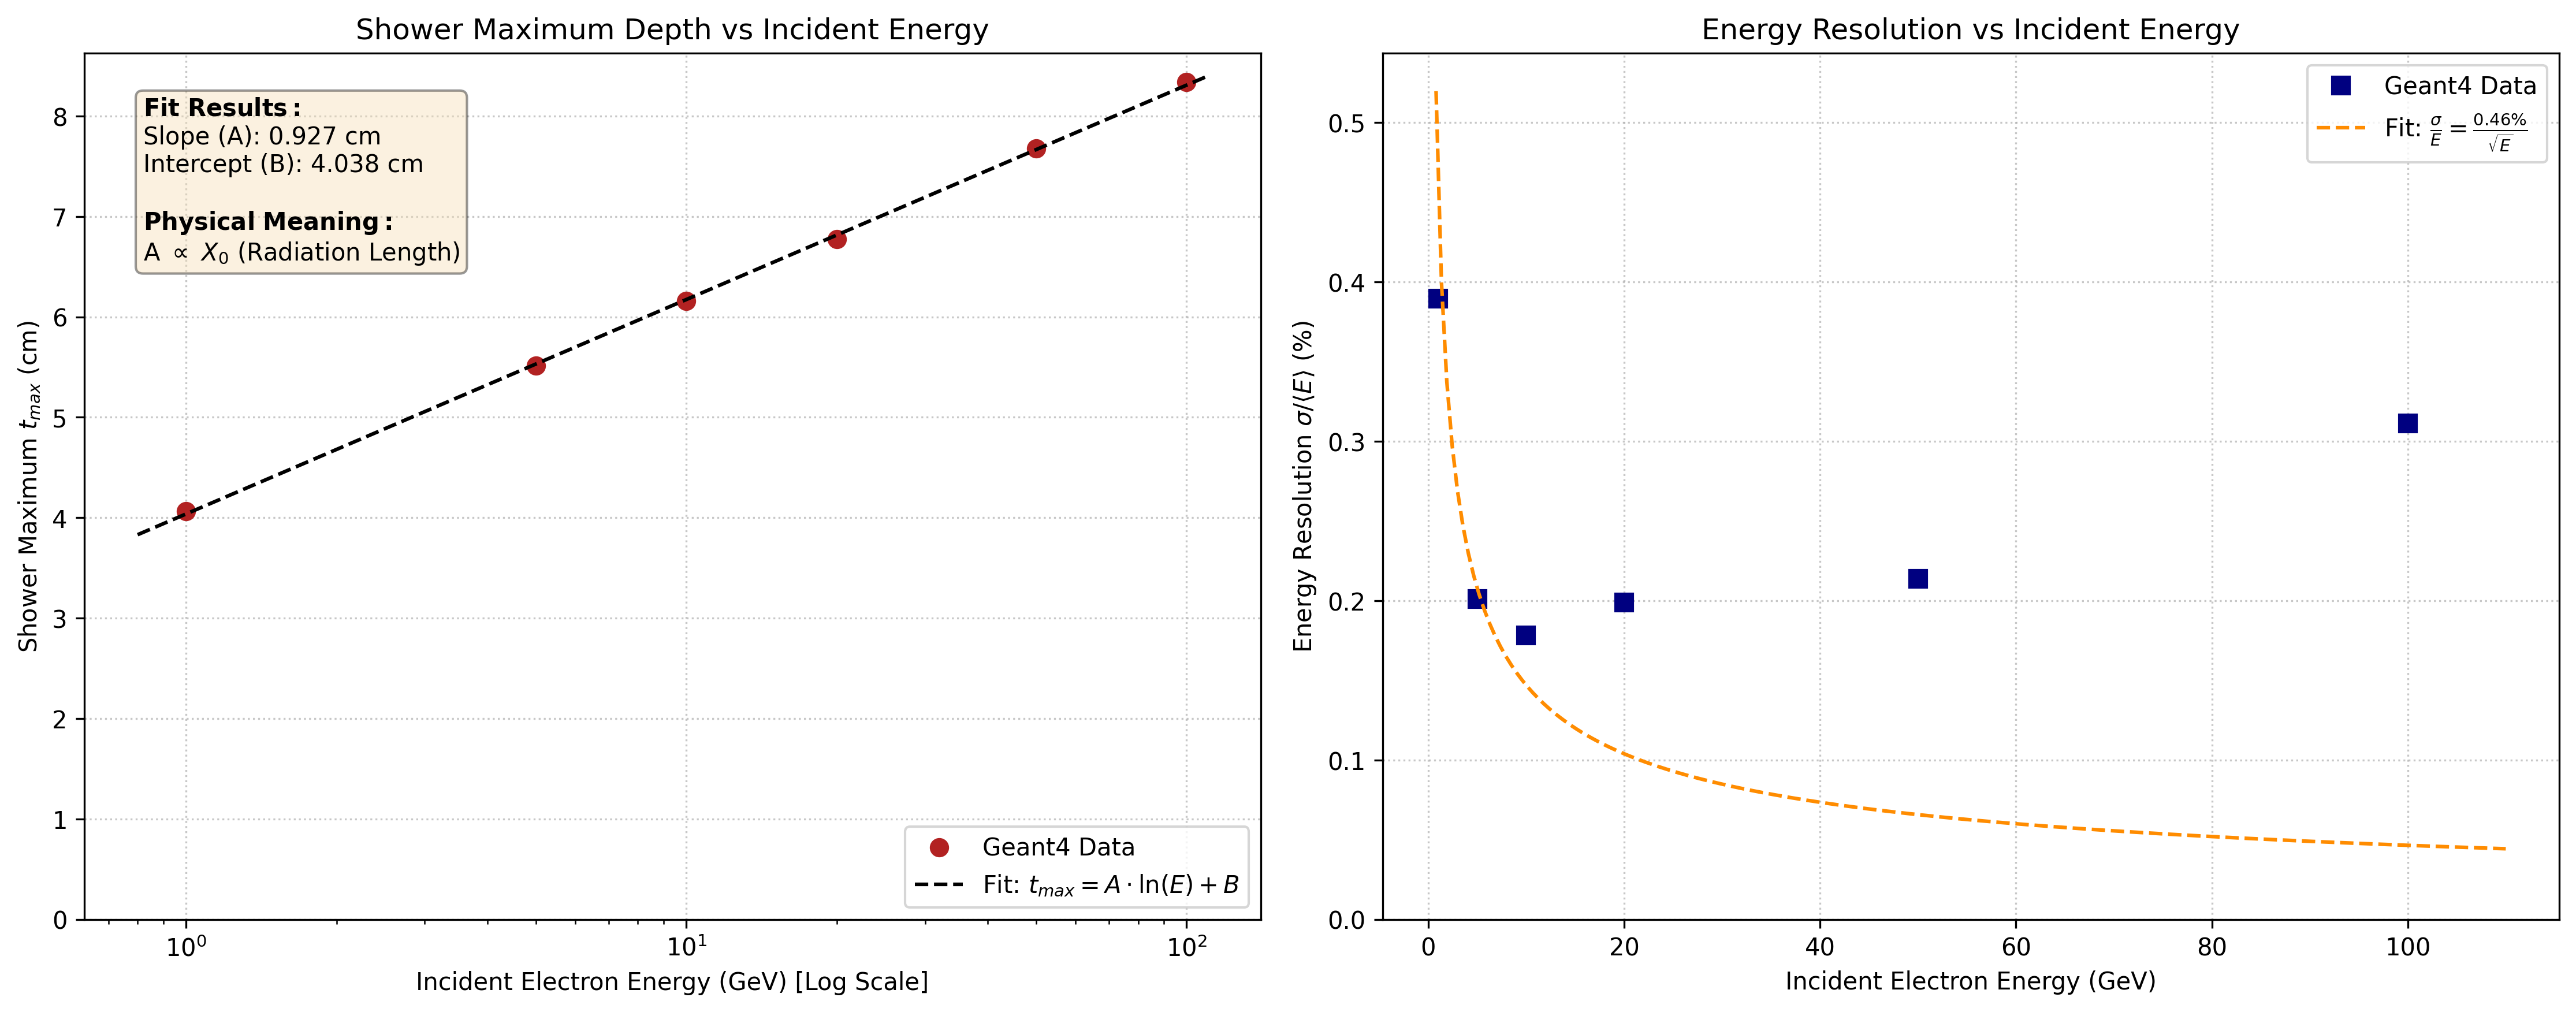
\includegraphics[width=0.9\textwidth, height=0.55\textheight, keepaspectratio]{Immagini/energy_response_analysis.png}
%    \end{figure}

%\end{frame}






% --- FRAME 1: Solo Grafico ---
\begin{frame}{Energy response: the resolution anomaly}

    \begin{figure}
        \centering
        % Sfruttiamo tutto lo spazio disponibile per il grafico
        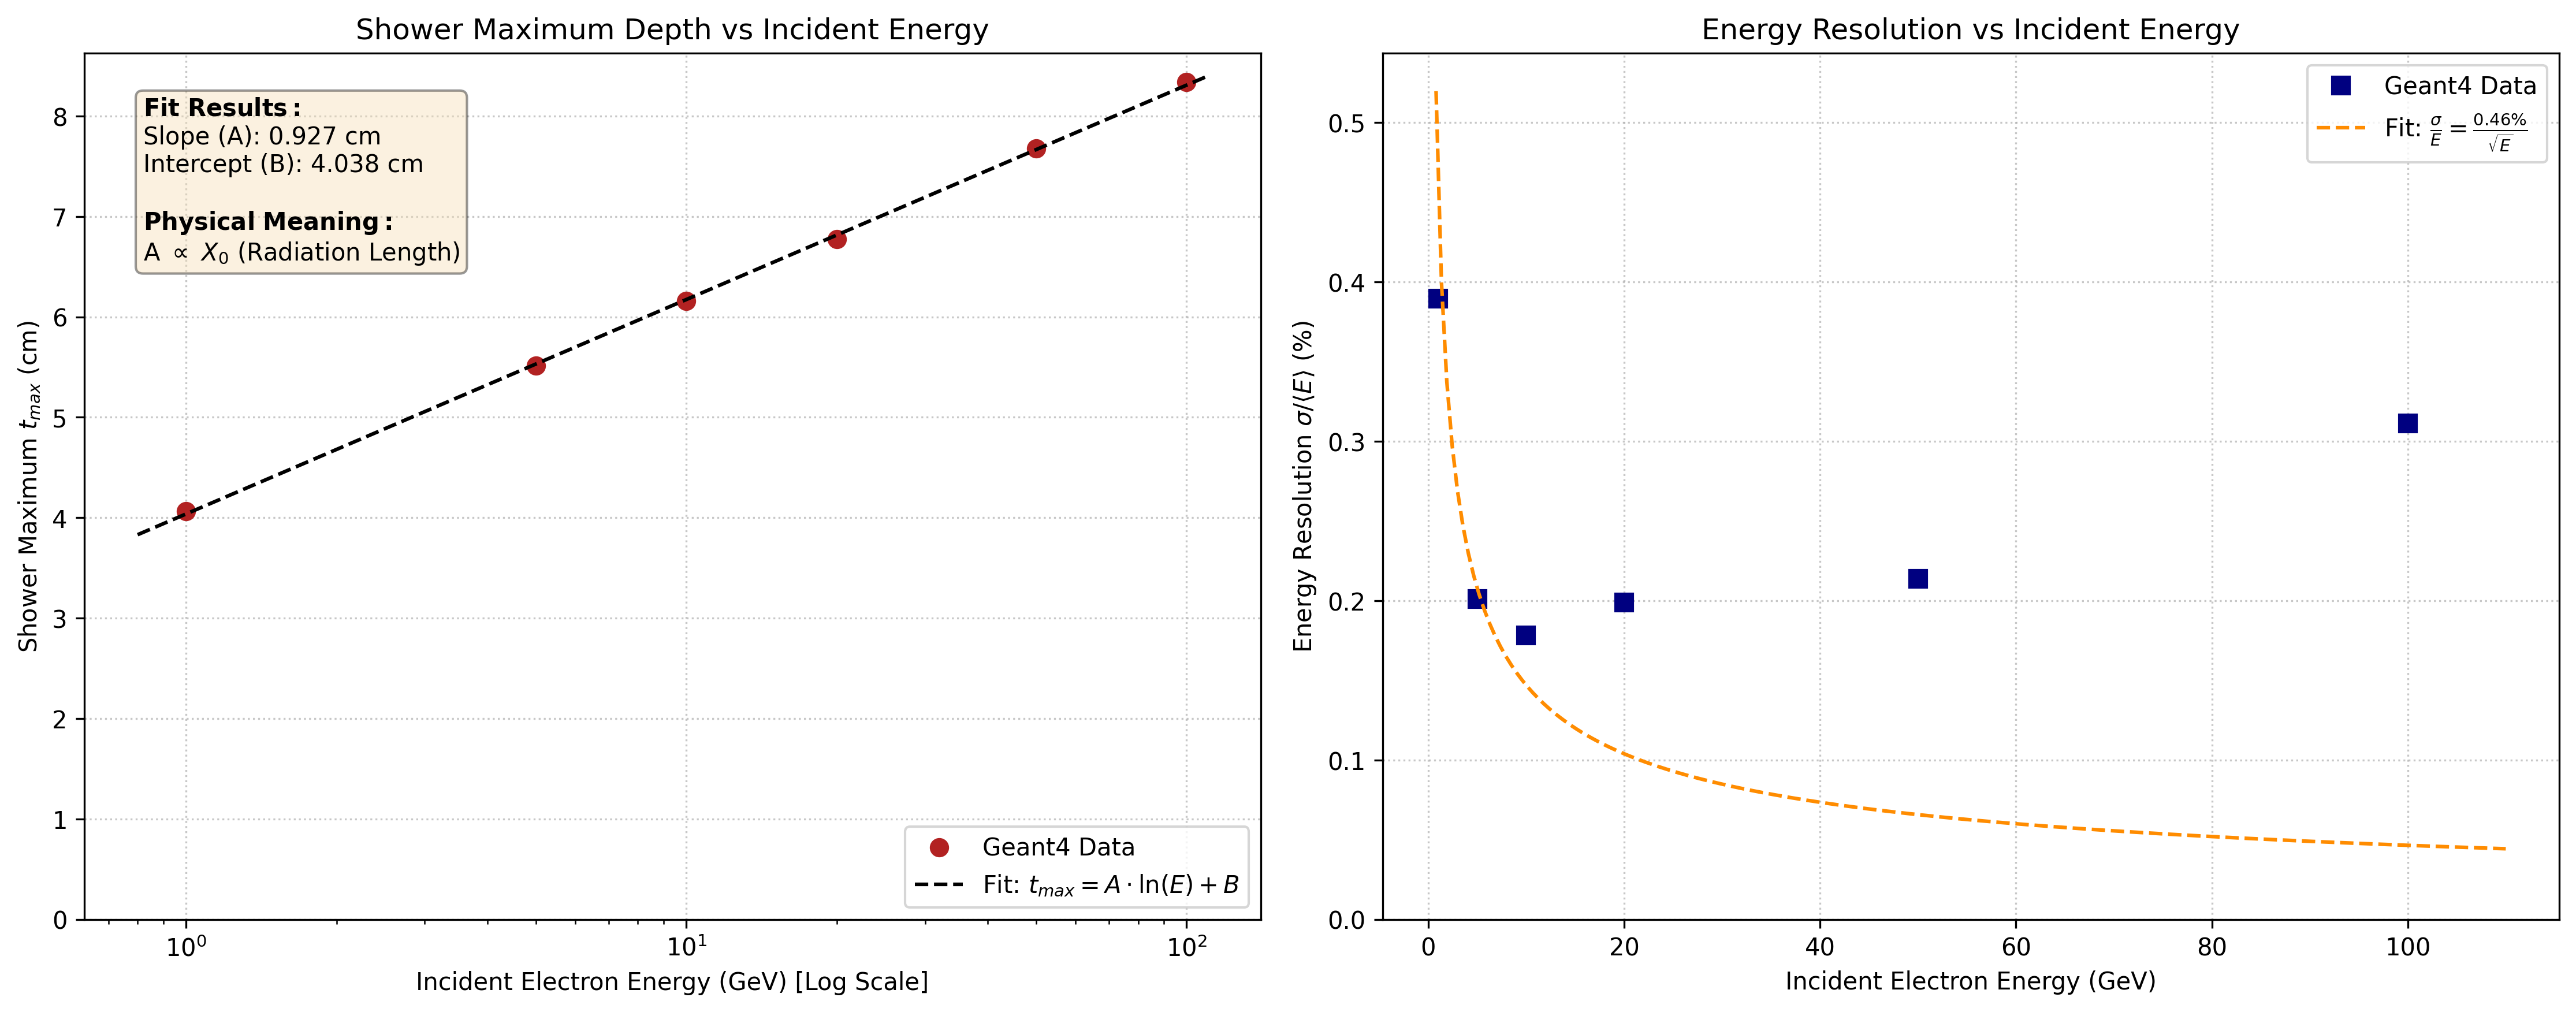
\includegraphics[width=0.95\textwidth, height=0.85\textheight, keepaspectratio]{Immagini/energy_response_analysis.png}
    \end{figure}

\end{frame}

% --- FRAME 2: Considerazioni Fisiche ---
\begin{frame}{Understanding the resolution anomaly}

    \begin{itemize}
        \item As predicted by cascade theory, the shower maximum ($t_{max}$) strictly scales with $\ln(E)$. 
        
        \vspace{0.3cm}
        
        \item Since the Geant4 simulation does not model photon production and collection inefficiencies, the intrinsic stochastic term is artificially tiny ($\sim 0.46\%/\sqrt{E}$).
        
        \vspace{0.3cm}
        
        \item Because this baseline intrinsic error is so close to zero, even minor event-by-event fluctuations caused by longitudinal leakage severely dominate the total resolution. This entirely breaks the ideal $1/\sqrt{E}$ scaling at high energies.
        
        \vspace{0.3cm}
        
        \item This effect is dramatically visible here, but it is usually masked in sampling calorimeters. In those setups, as we will see later, the inherently large sampling fluctuations ($\approx 10\%/\sqrt{E}$) easily cover up these small leakage penalties.
    \end{itemize}

\end{frame}




\begin{frame}{Sampling calorimeter dimensioning (Pb/LAr)}
    \begin{columns}[T]
        
        % Left Column: Theory & Setup (45% width)
        \begin{column}{0.47\textwidth}
            \vspace{0.2cm}
            Simulating 100 GeV electrons.\\ 
            The setup uses $50$ layers with a 3:4 thickness ratio for Pb and LAr respectively.
            
            \begin{itemize}
                \item $X_0(\text{Pb}) = 0.56\,\text{cm}$
                \item $X_0(\text{LAr}) = 14.0\,\text{cm}$
            \end{itemize}
            \vspace{-0.2cm}

            $$ X_{\text{eff}} = 1.24\,\text{cm} \qquad \text{Depth} \approx 25 X_{\text{eff}} = 31\,\text{cm} $$
                        \vspace{-0.2cm} 

        \end{column}
        
        % Right Column: Simulation Result (55% width)
        \begin{column}{0.53\textwidth}
            \begin{figure}
                \centering
                % Assicurati che il nome e il percorso del file siano corretti
                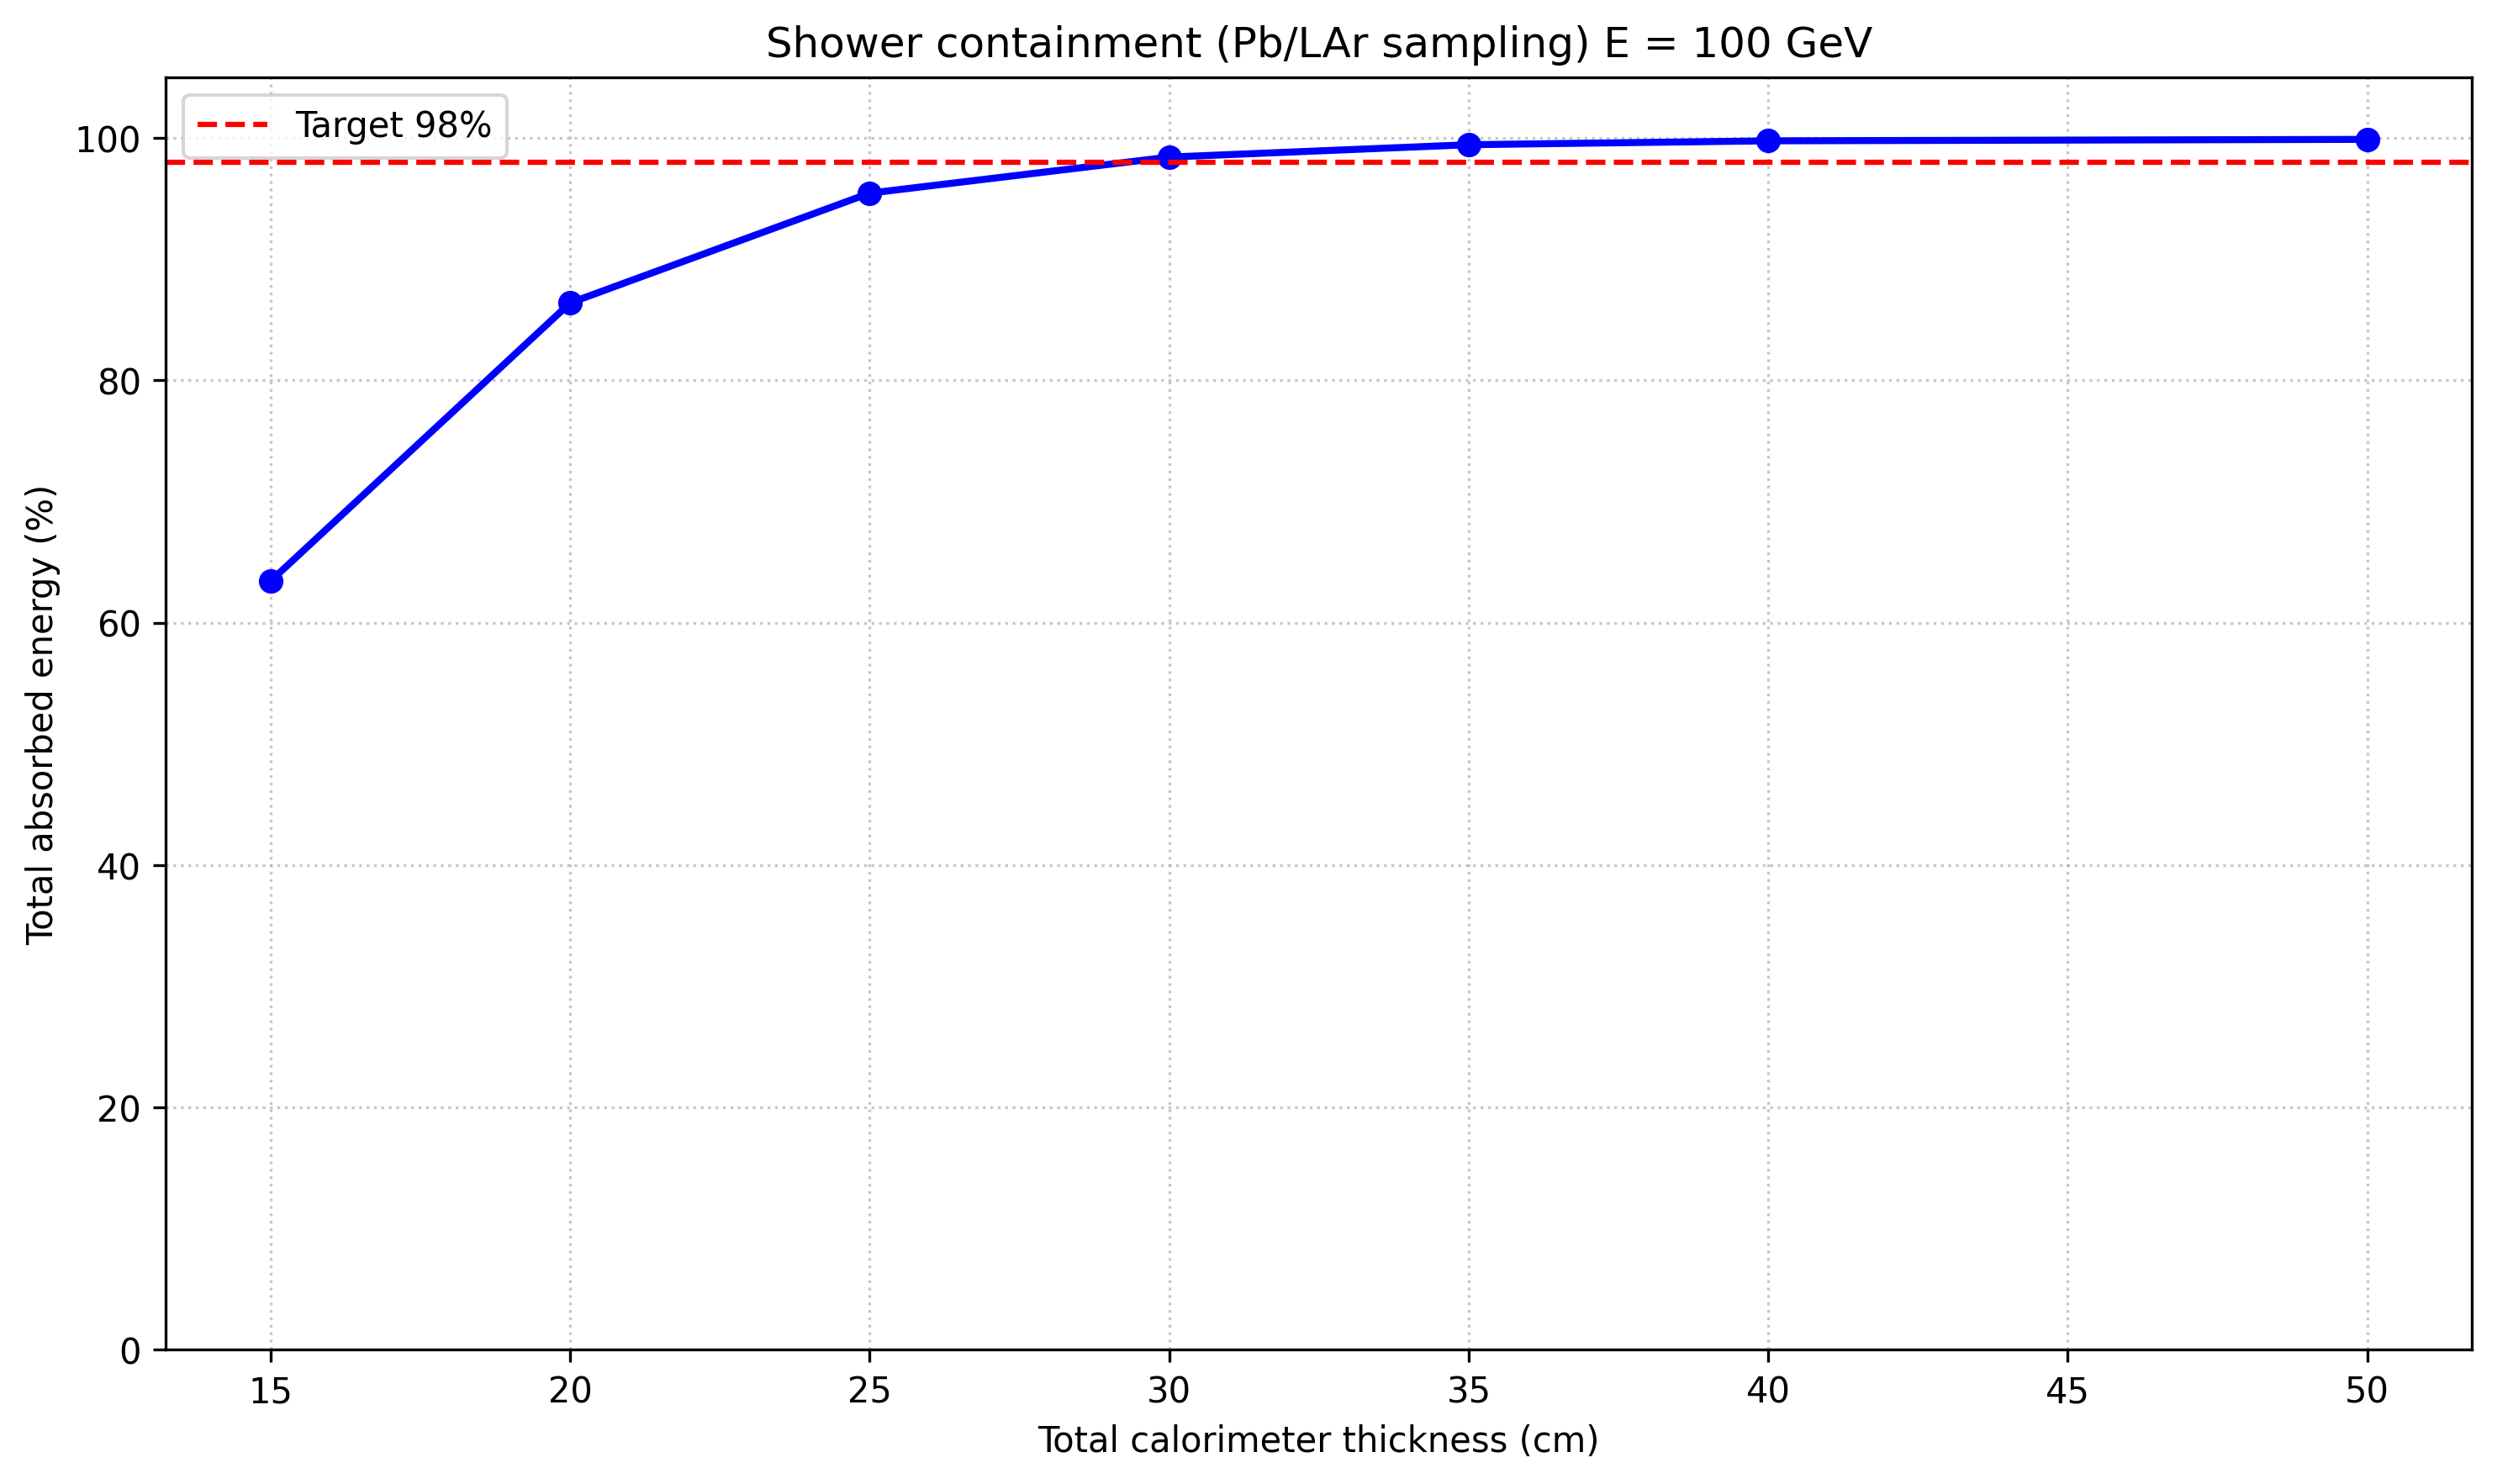
\includegraphics[width=\textwidth, keepaspectratio]{Immagini/sampling_containment_results.png} 
            \end{figure}
        \end{column}
    \end{columns}
                
        The simulation confirms the $98\%$ absorbed energy threshold is successfully reached at $30\,\text{cm}$ of total thickness.
\end{frame}

\begin{frame}{Effect of upstream dead material (sampling)}

        The unmeasured energy absorbed by the dead material fluctuates event-by-event, severely degrading the sampling resolution.
        
    \begin{figure}
        \centering
        % Sostituisci con il nome esatto del tuo file immagine
        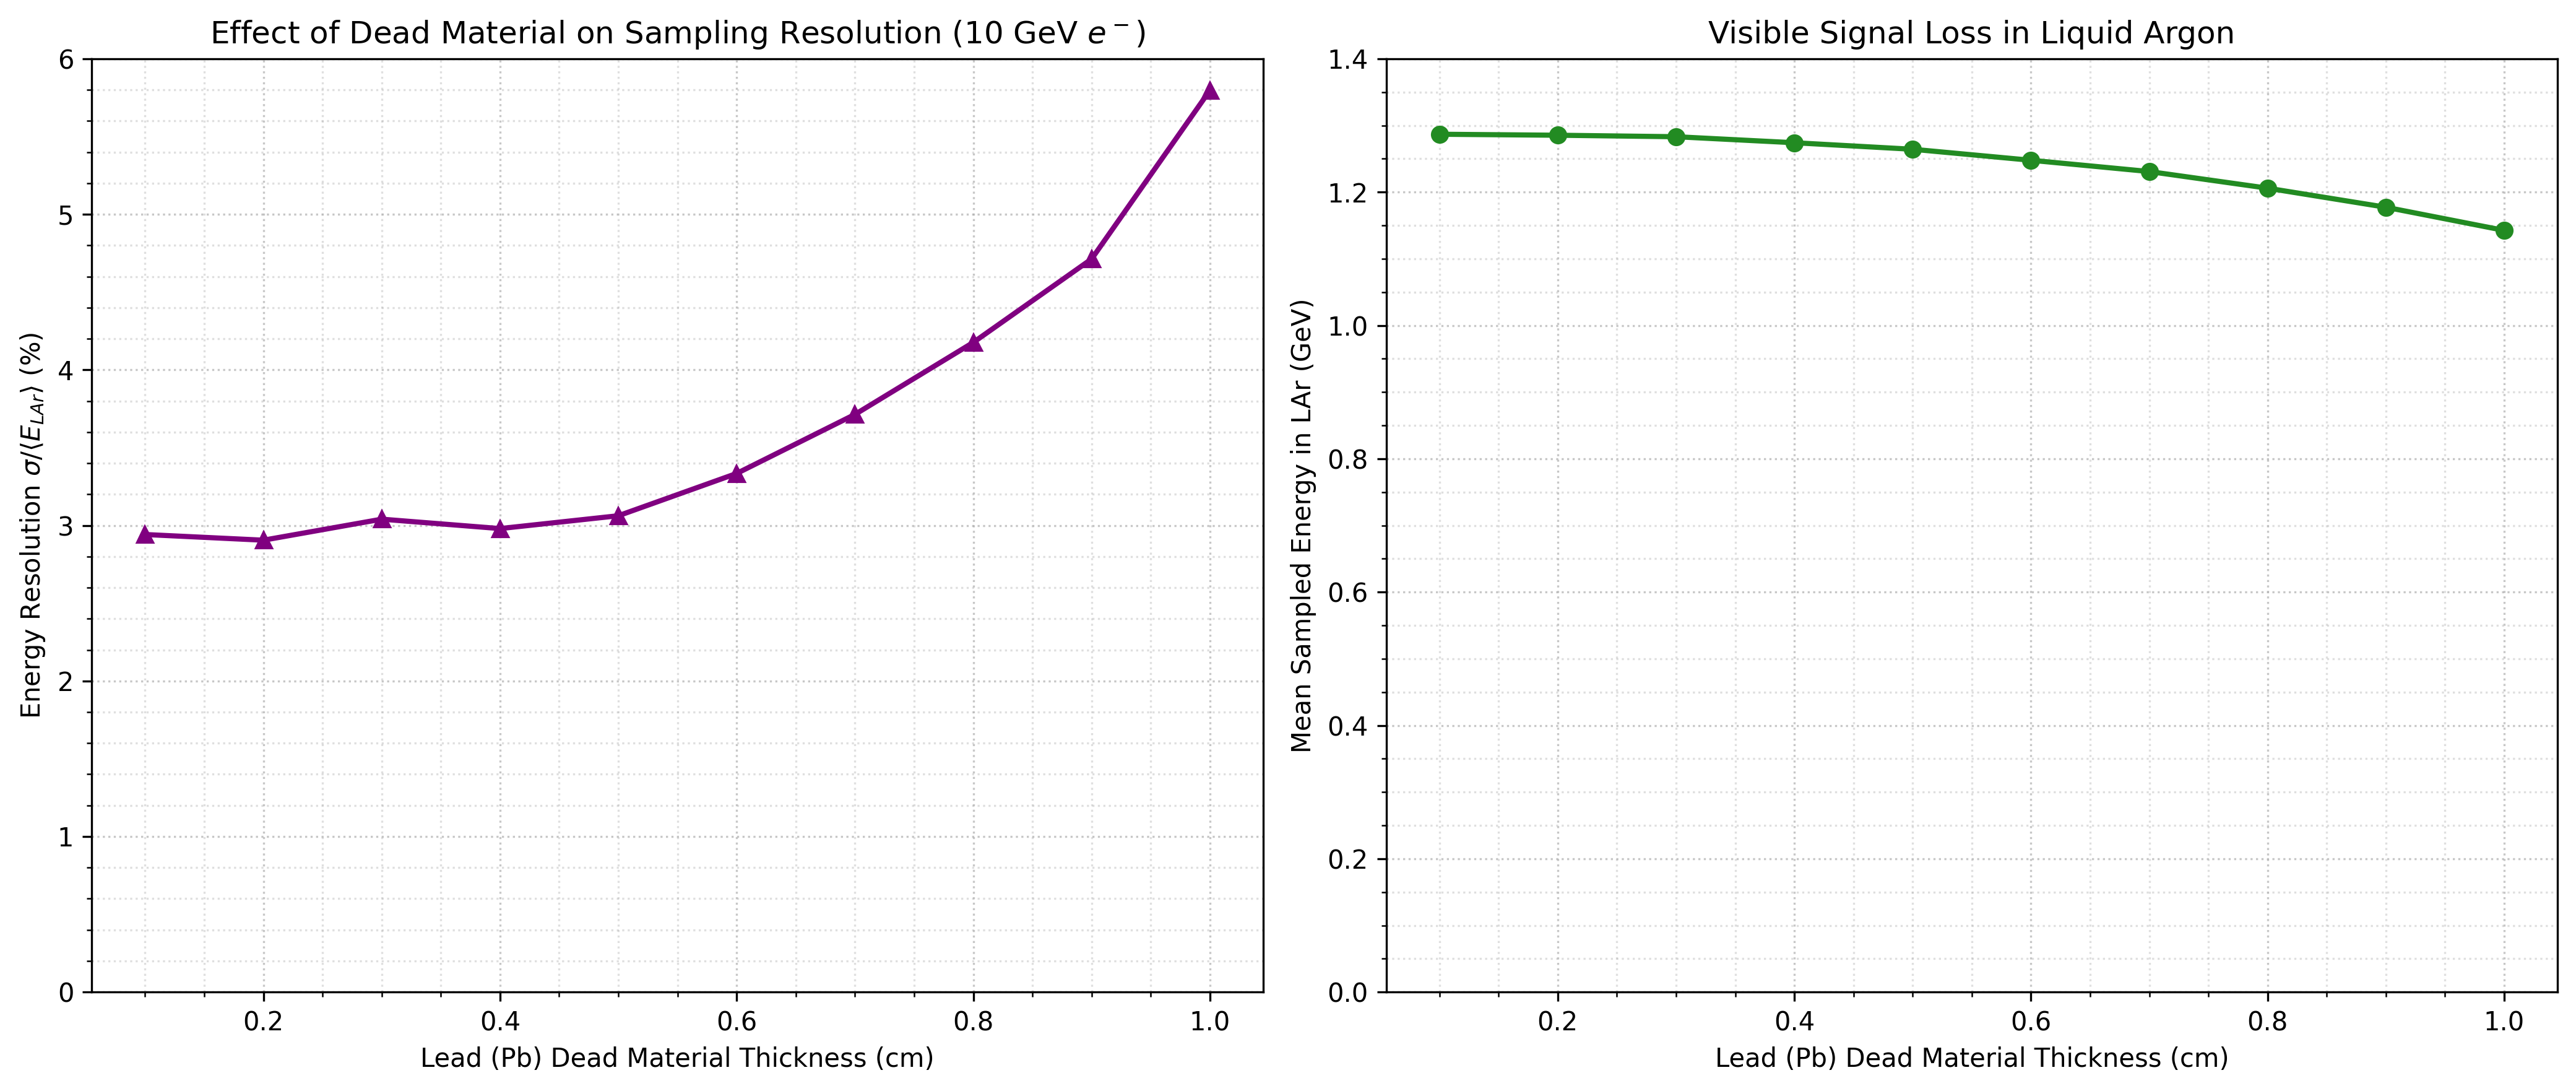
\includegraphics[width=0.9\textwidth, keepaspectratio]{Immagini/dead_material_sampling.png}
    \end{figure}

\end{frame}

\begin{frame}{Optimal cell size: transverse containment (Pb/LAr)}
    \begin{columns}[T]
        
        % Left Column: Minimal Theory (35% width)
        \begin{column}{0.35\textwidth}
            \begin{itemize}
                \item Cell size is determined by the 87\% transverse energy containment limit.
                \item The data shows an effective radius of $R_M = 3.12\,\text{cm}$.
            \end{itemize}
        \end{column}
        
        % Right Column: Graph (65% width)
        \begin{column}{0.65\textwidth}
            \begin{figure}
                \centering
                % Assicurati che il percorso del file sia corretto
                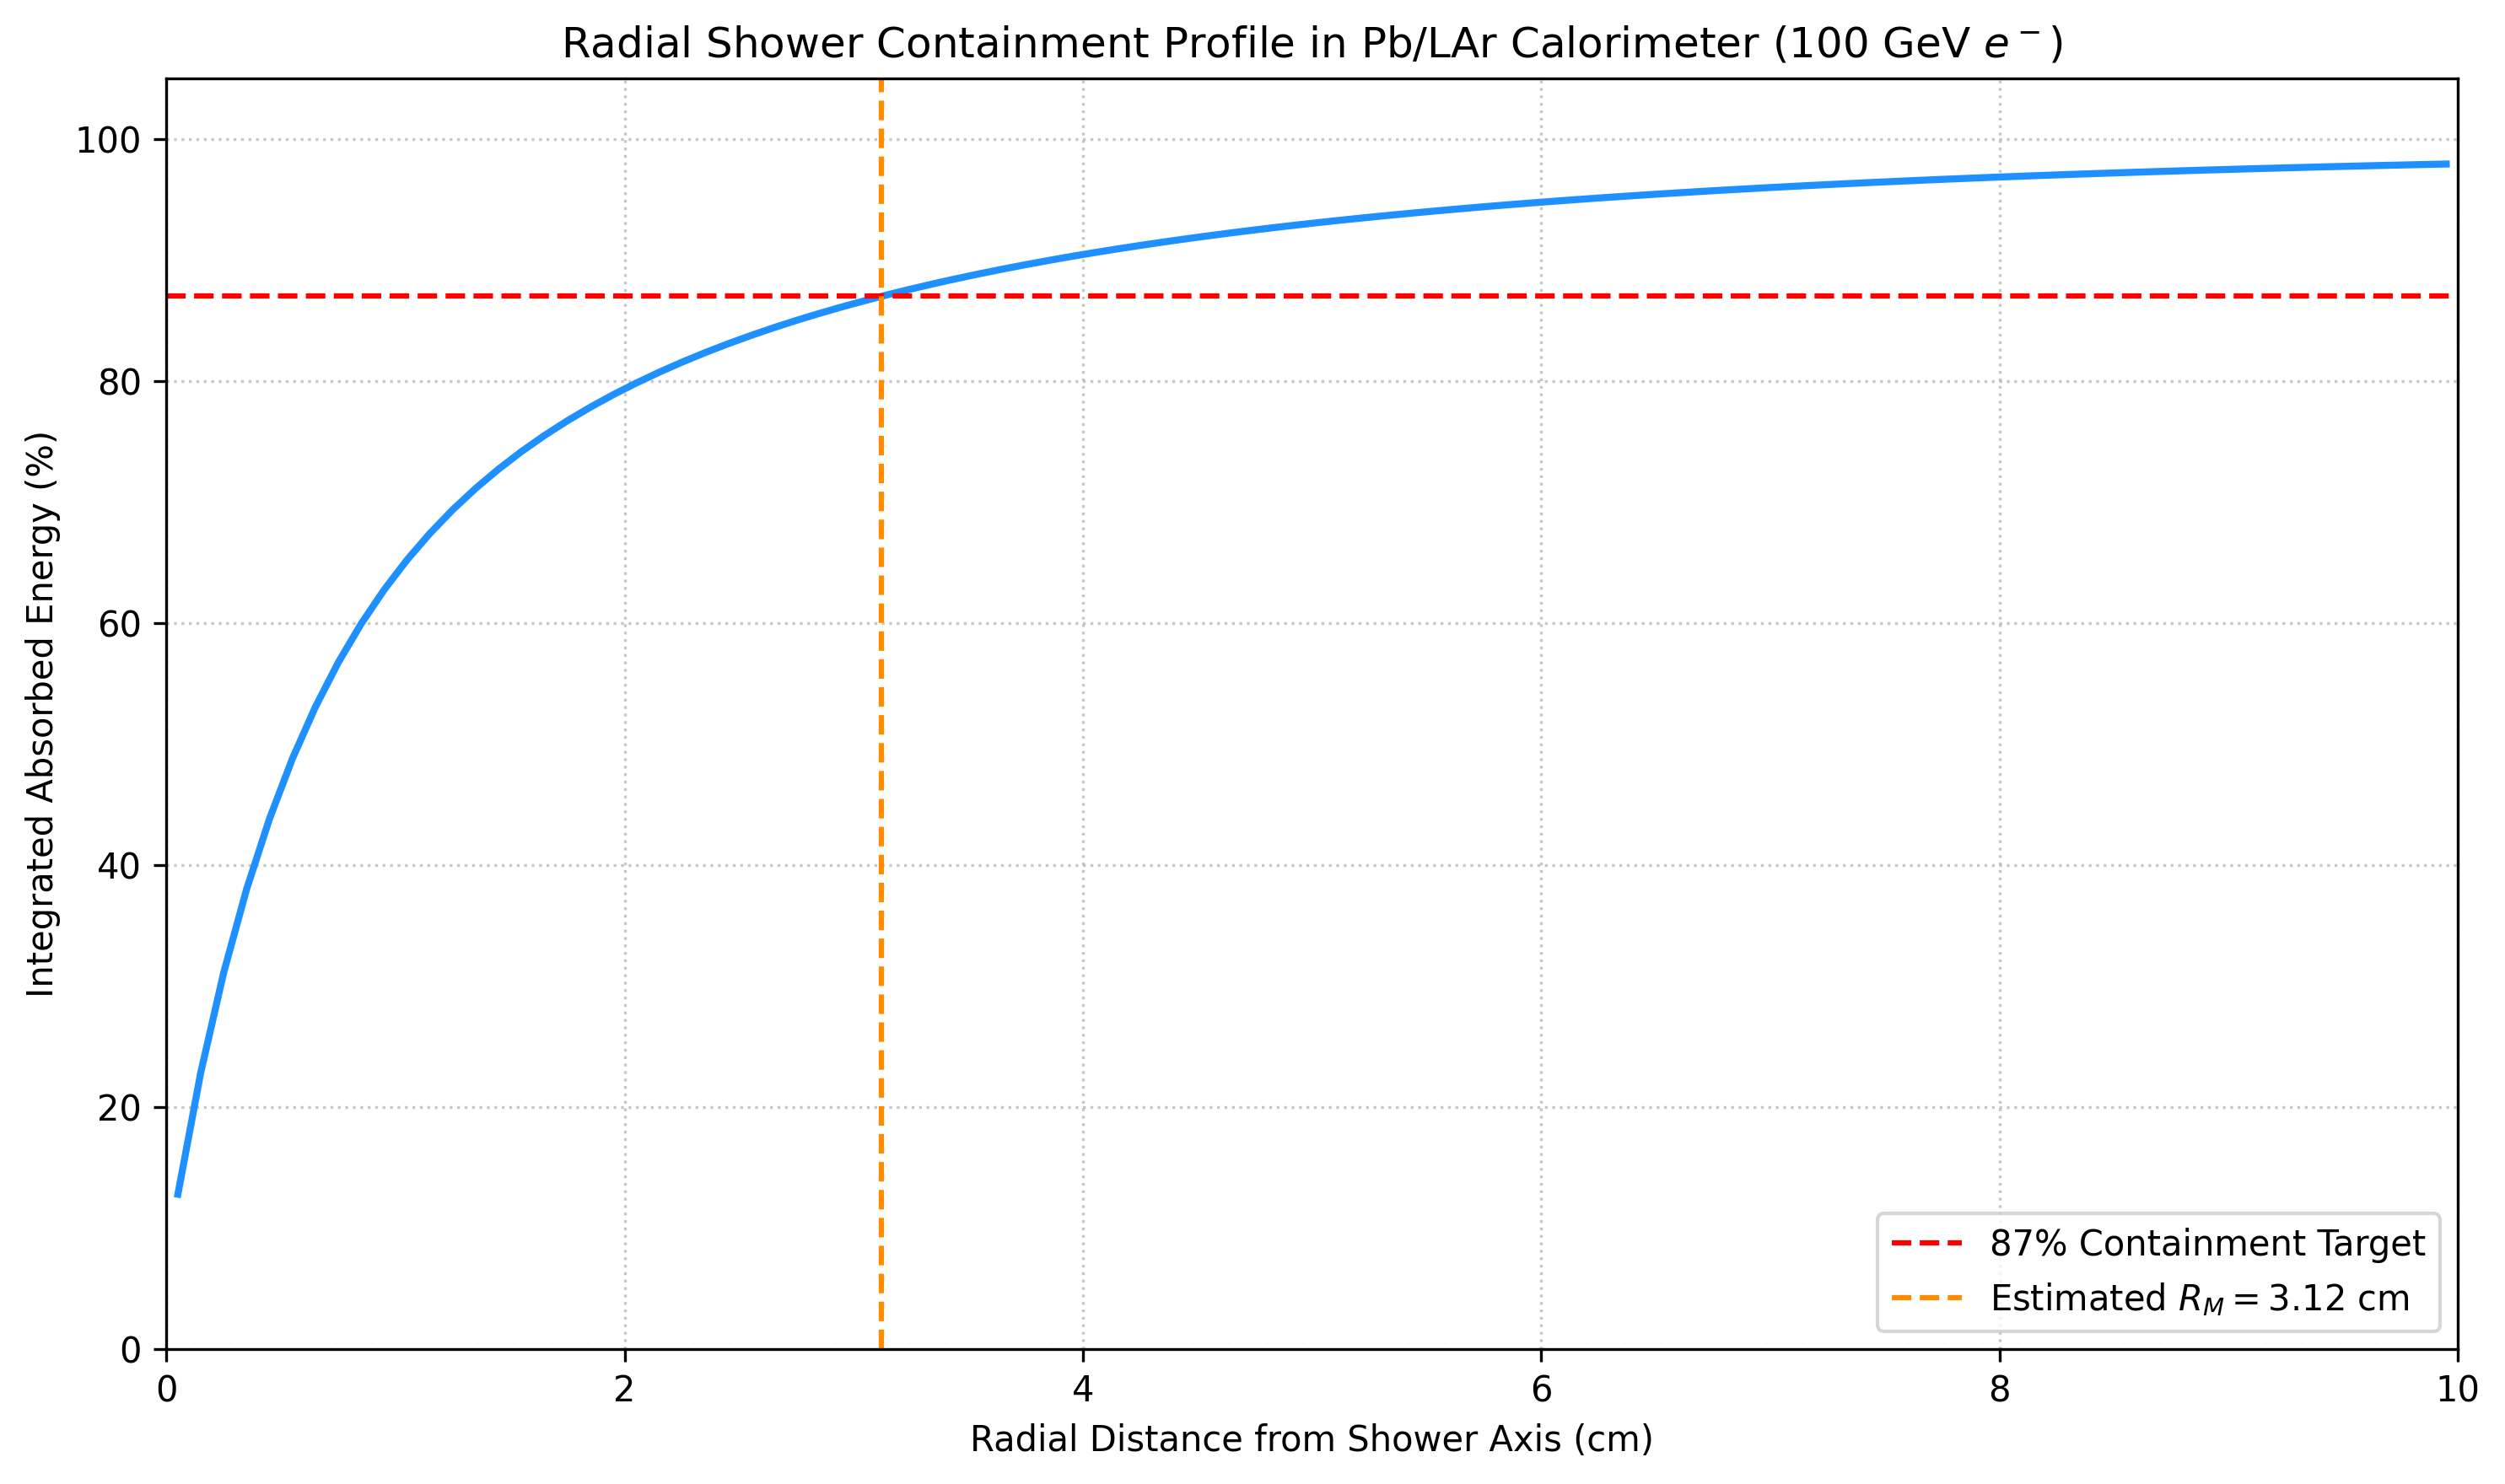
\includegraphics[width=\textwidth, keepaspectratio]{Immagini/radial_containment_samp.png}
            \end{figure}
        \end{column}
        
    \end{columns}
\end{frame}
\begin{frame}{Sampling frequency \& energy resolution}

    Fixed total material ($15\,\text{cm}$ Pb + $20\,\text{cm}$ LAr). Layers varied from $100$ down to $10$. Thicker individual Pb absorbers reduce sampling frequency, worsening the energy resolution.
    
    
    \begin{figure}
        \centering
        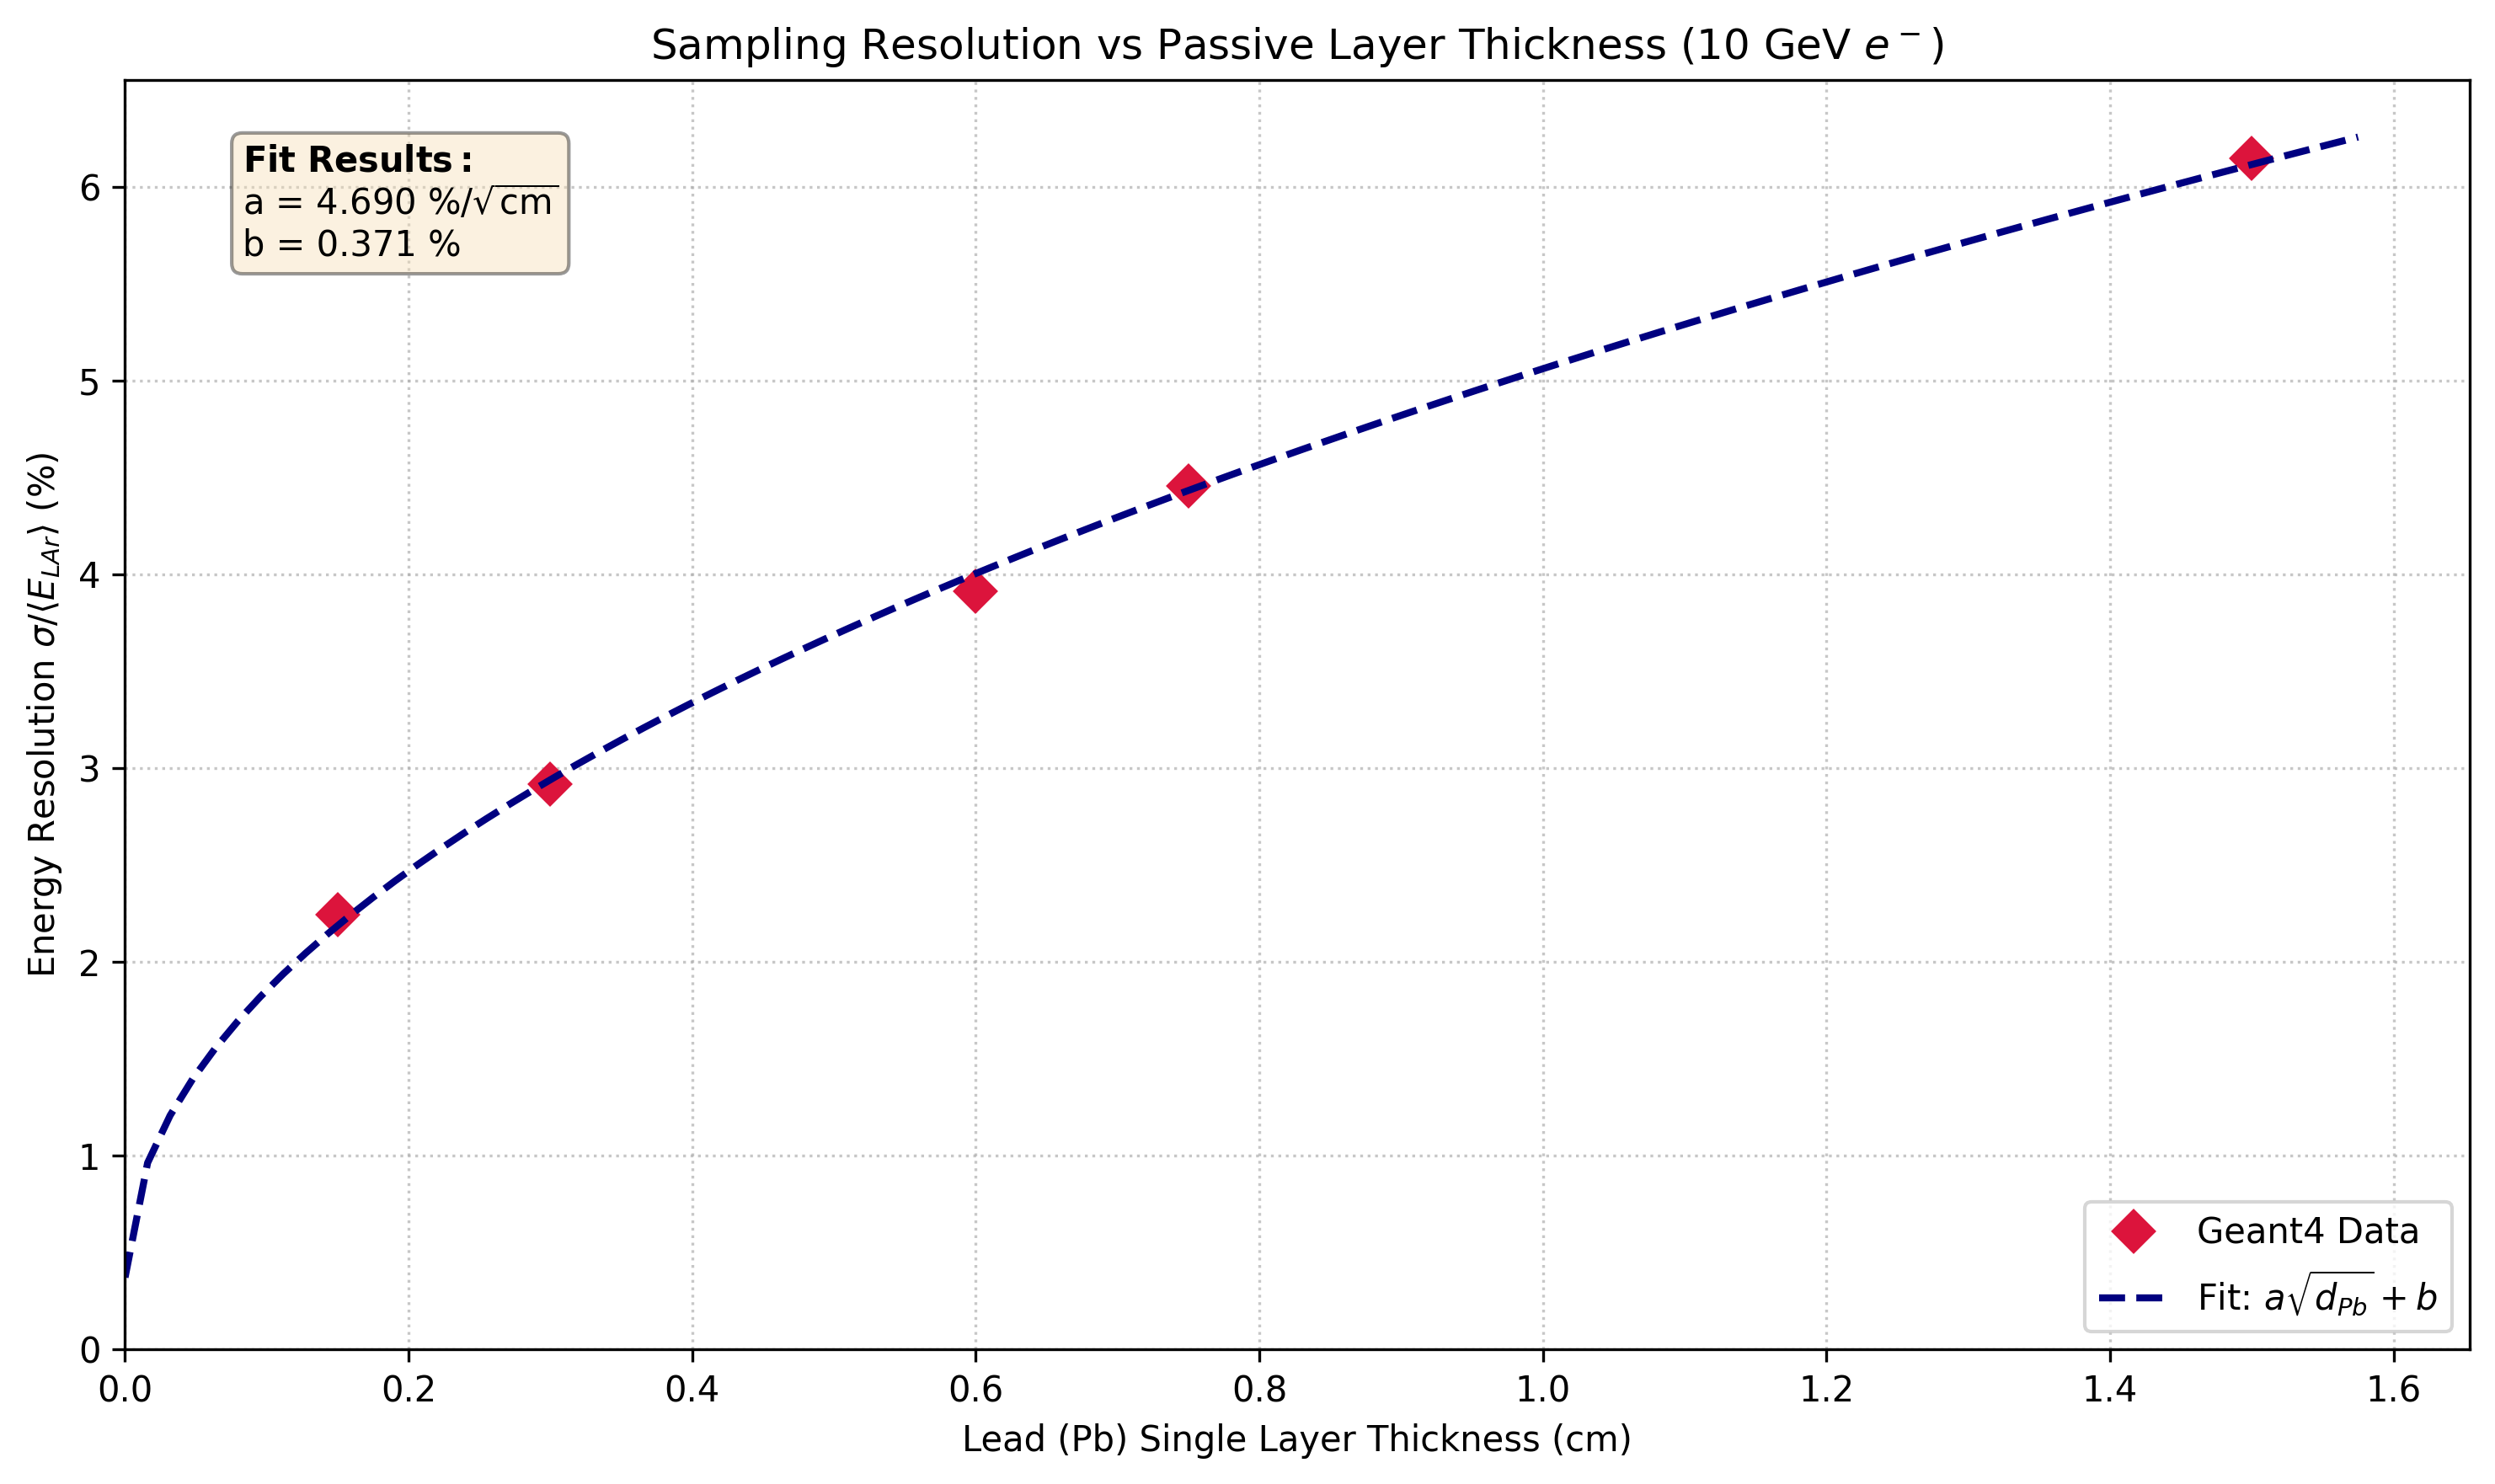
\includegraphics[width=0.65\textwidth, keepaspectratio]{Immagini/sampling_frequency_resolution.png}
    \end{figure}

\end{frame}

\begin{frame}{Sampling calorimeter response (1--100 GeV)}

    As expected from cascade models, the penetration depth $t_{max}$ strictly follows a logarithmic scaling with energy $\ln(E)$. \\
    The energy resolution shows an excellent agreement with the stochastic term $\sigma/E = a/\sqrt{E}$. 
    
    
    \begin{figure}
        \centering
        % Assicurati che il percorso del file sia corretto
        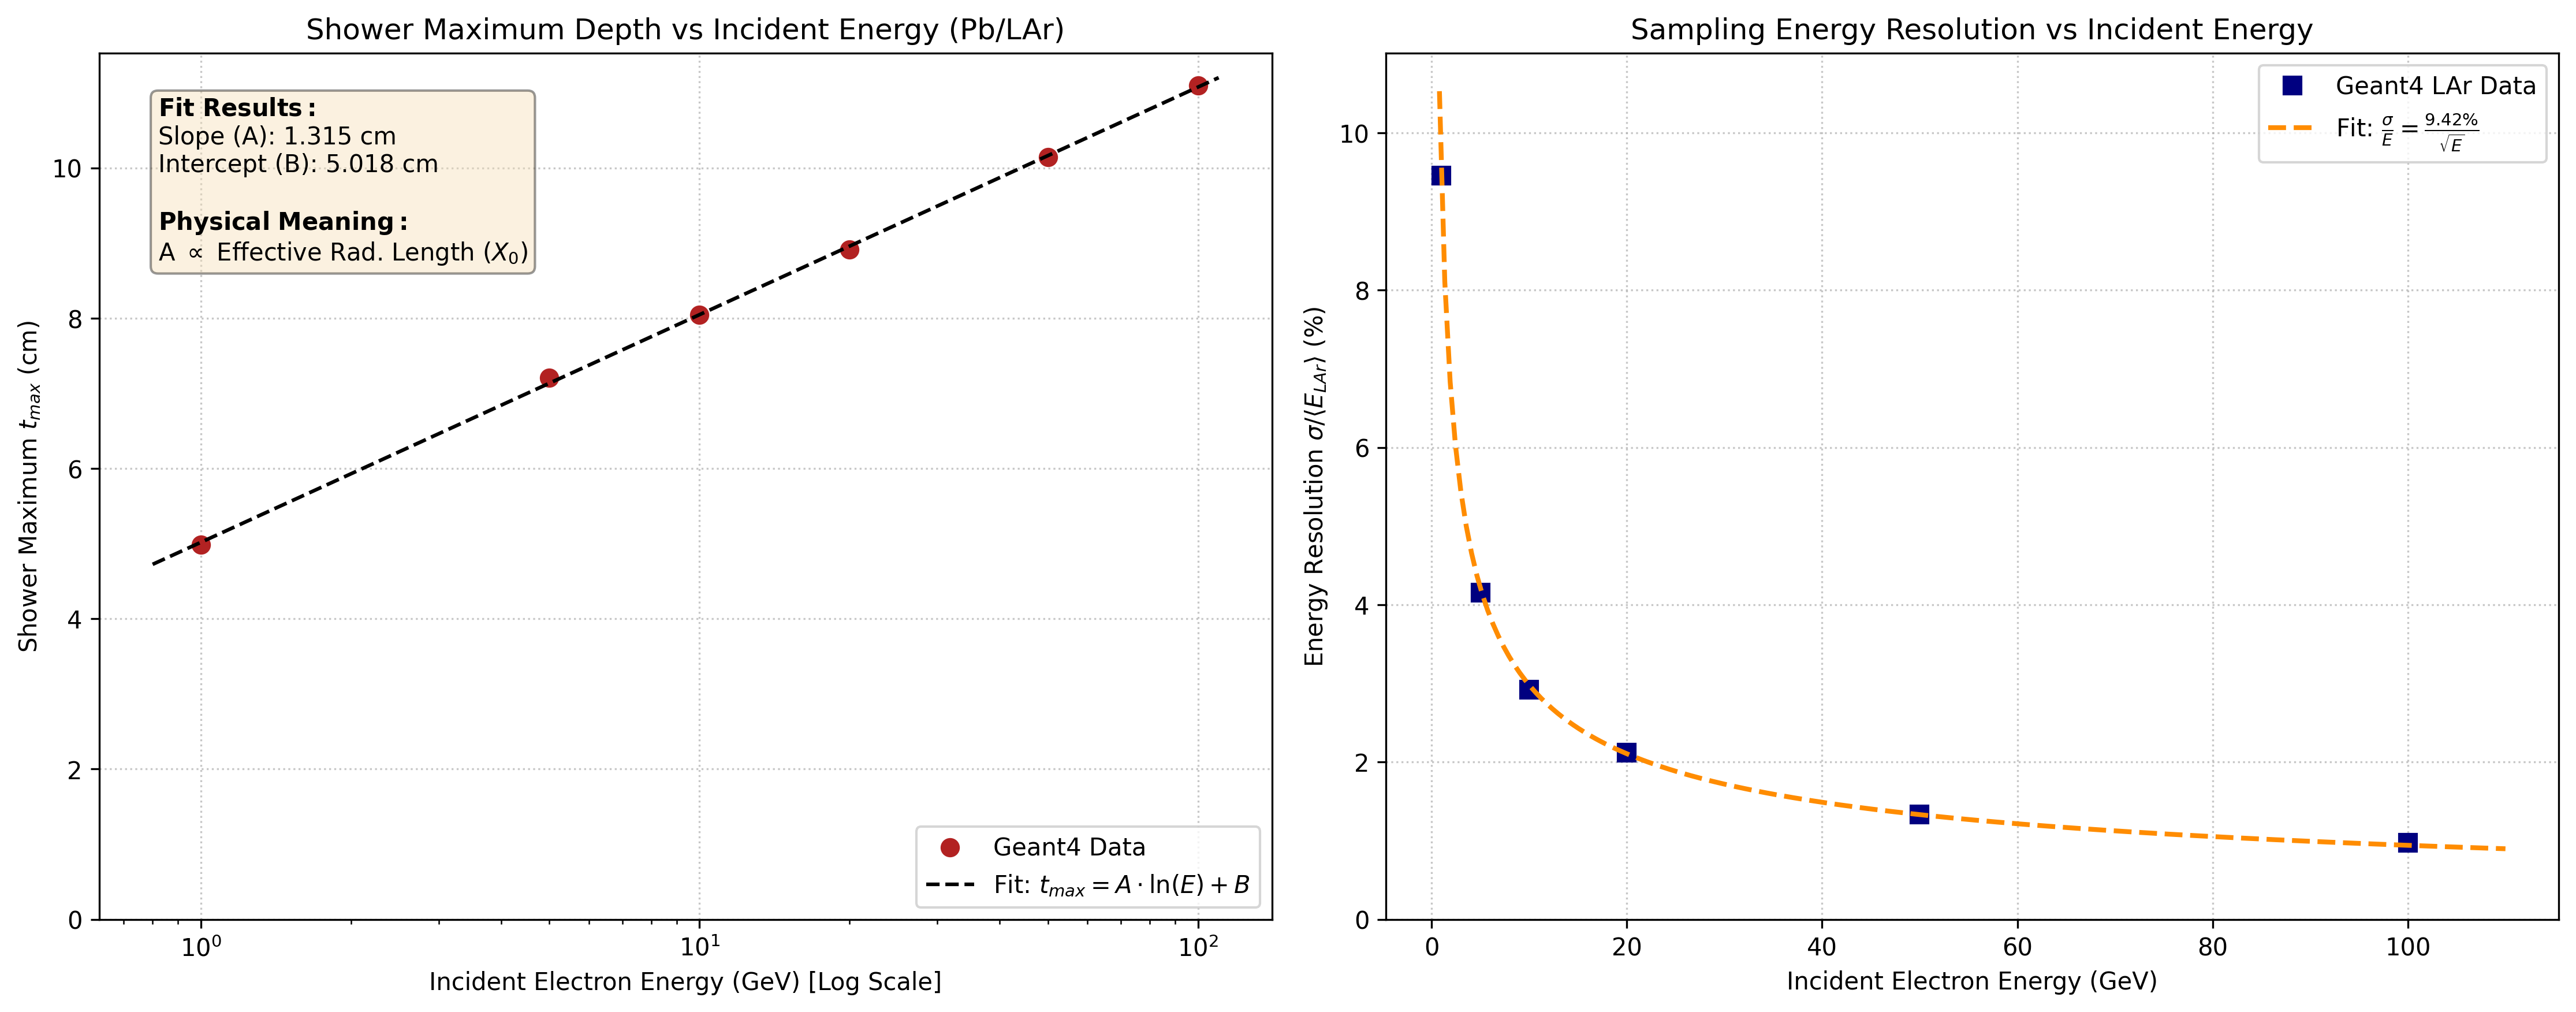
\includegraphics[width=0.92\textwidth, height=0.70\textheight, keepaspectratio]{Immagini/sampling_energy_response.png}
    \end{figure}

\end{frame}

\begin{frame}{Muon energy response (Pb/LAr)}

    Up to $\sim 100\,\text{GeV}$, muons act as Minimum Ionizing Particles (MIPs), depositing a small and nearly constant fraction of their energy via ionization. \\
    At ultra-high energies ($500\text{--}1000\,\text{GeV}$), radiative losses (e.g., bremsstrahlung) become dominant, causing a sharp increase in the deposited energy.    
    \begin{figure}
        \centering
        % Assicurati che il percorso del file sia corretto
        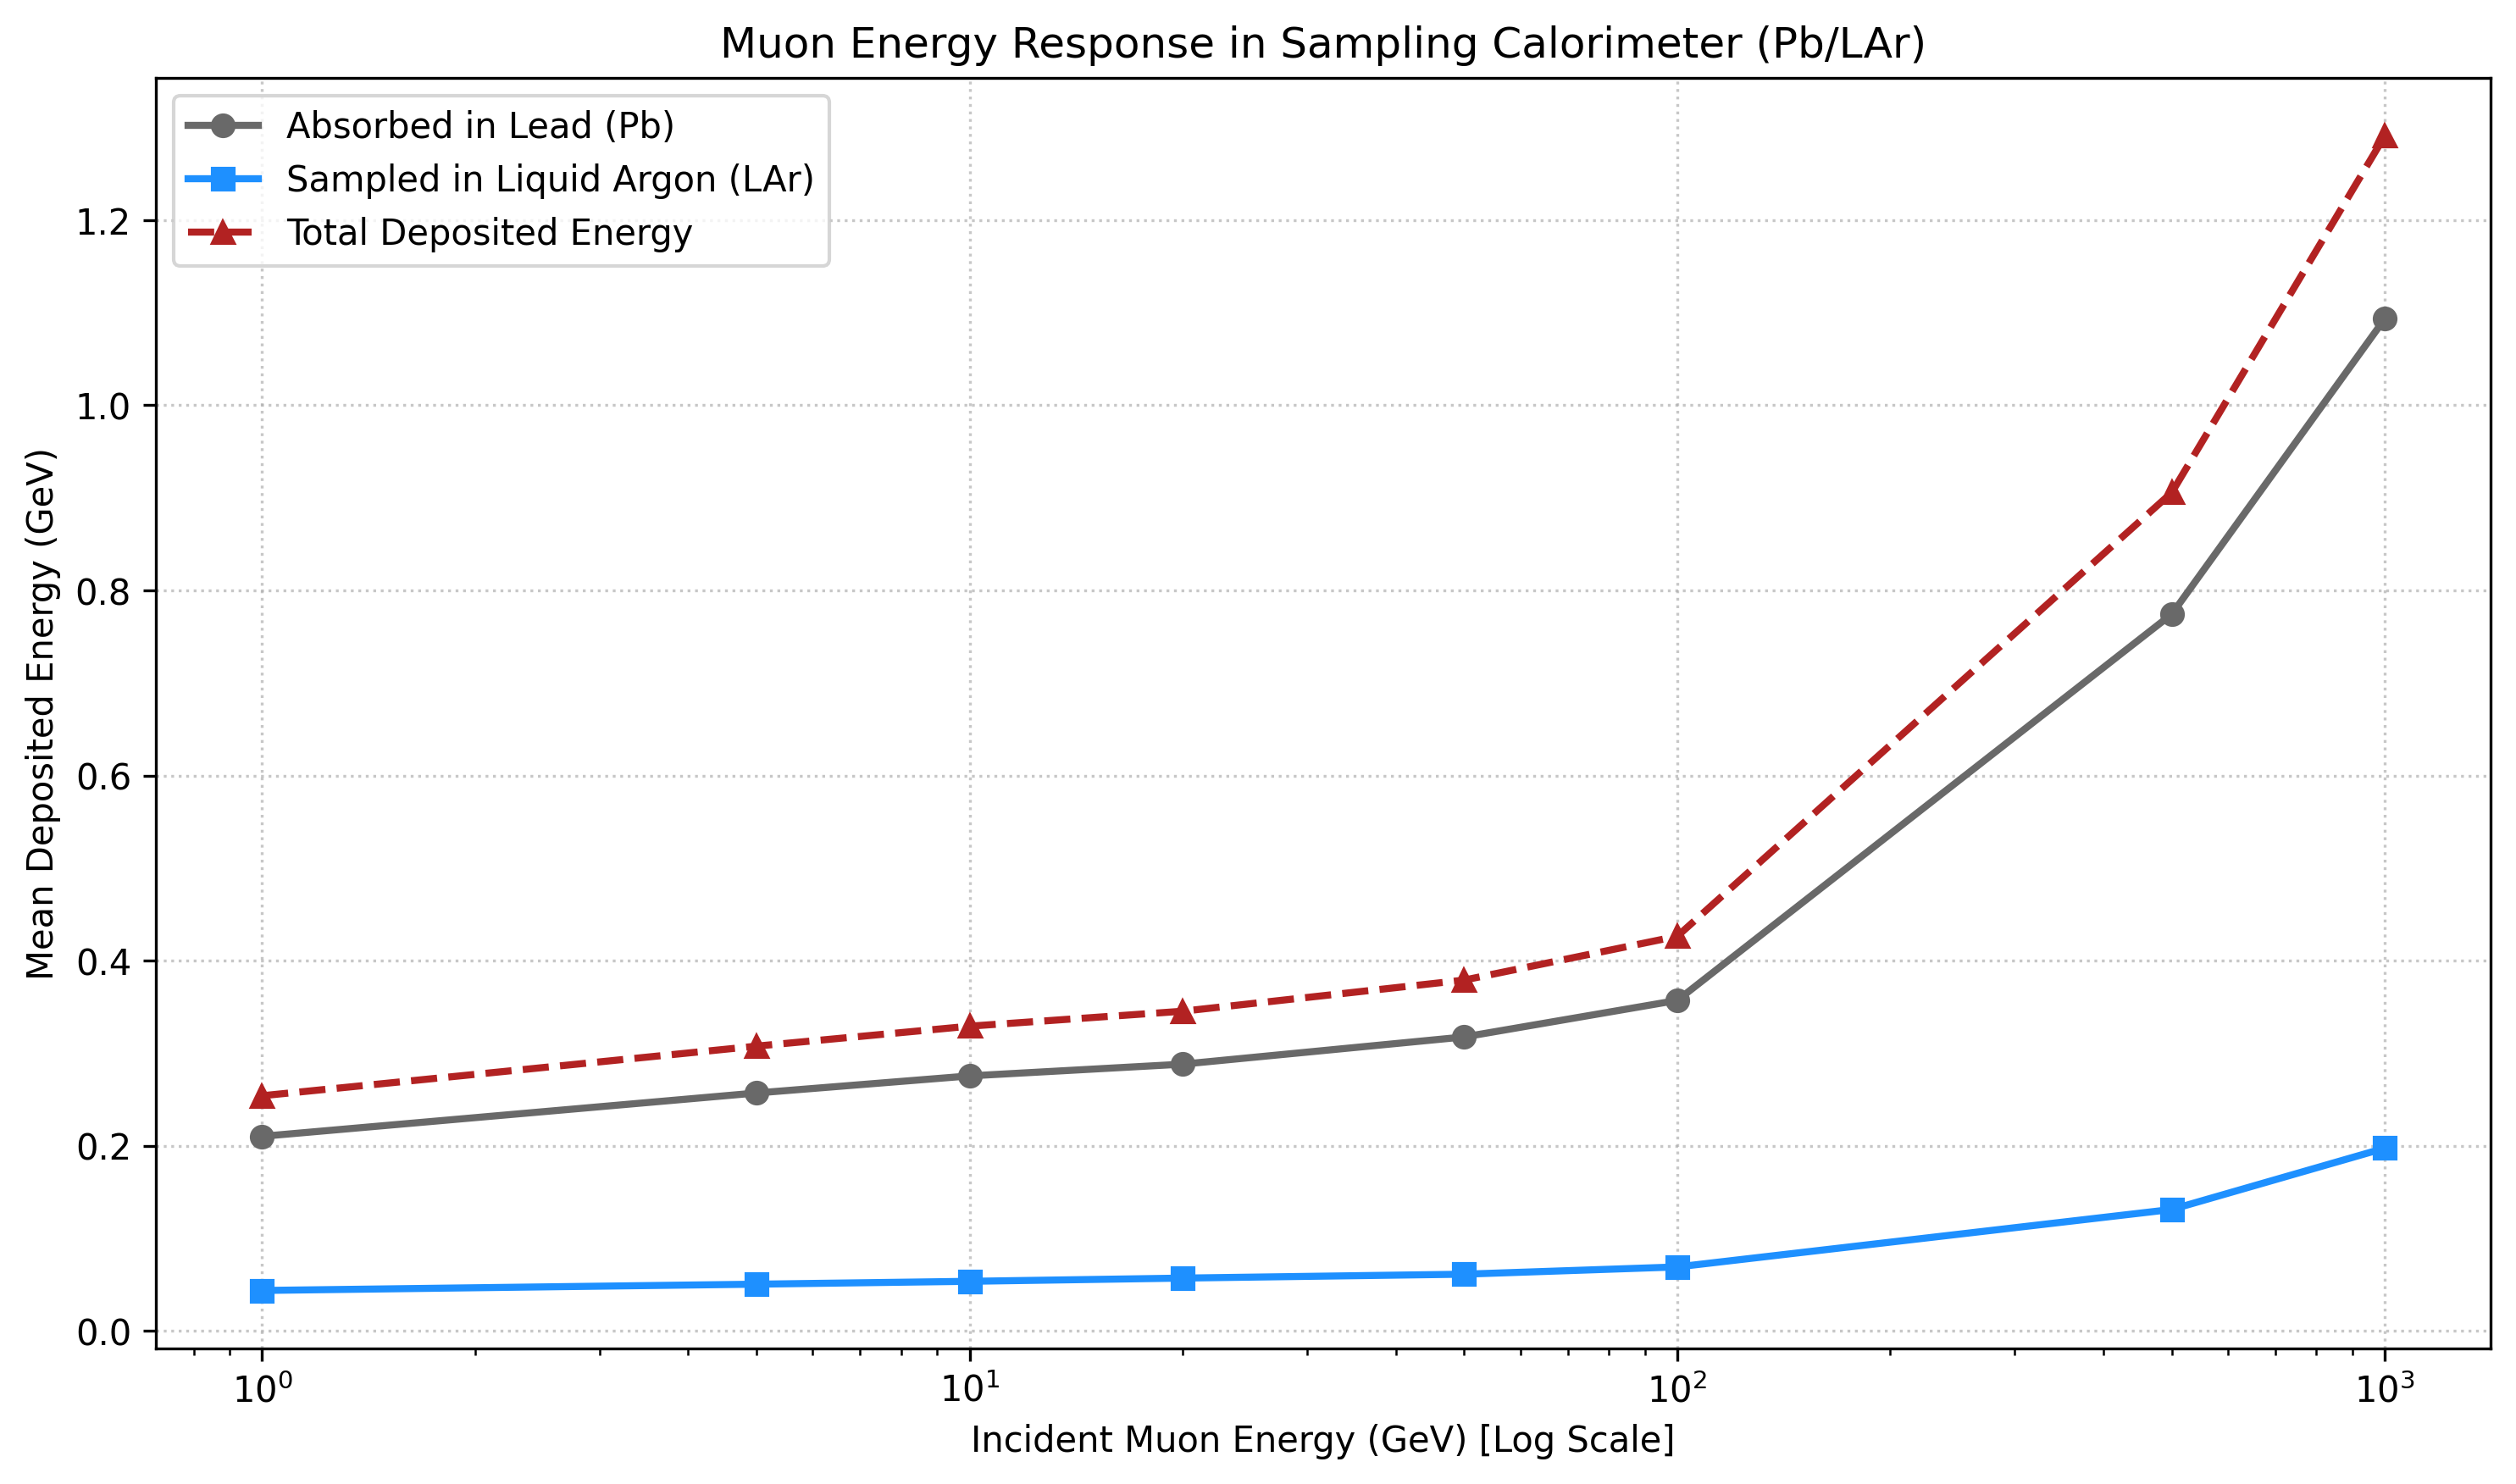
\includegraphics[width=0.95\textwidth, height=0.68\textheight, keepaspectratio]{Immagini/muon_response_analysis.png}
    \end{figure}

\end{frame}

% ==================///==================///==================///
% ==================/// END PRESENTATION
% ==================///==================///==================///

\backmatter

\appendix
\section*{BACKUP}
\begin{frame}[noframenumbering]
    \begin{center}
        \Huge \textbf{BACKUP}
    \end{center}
\end{frame}

% --- BACKUP SLIDE 1 ---
\begin{frame}[noframenumbering]{Resolving the resolution anomaly}

    In a pure Geant4 simulation lacking photon collection inefficiencies and electronic noise, the intrinsic stochastic term is extremely small. Therefore, even minor event-by-event fluctuations caused by longitudinal leakage become the dominant source of error at high energies, breaking the ideal $\propto 1/\sqrt{E}$ scaling. By doubling the $PbWO_4$ detector length to $50\,\text{cm}$, the shower tail is fully contained.
    \vspace{-0.2cm}
    \begin{figure}
        \centering
        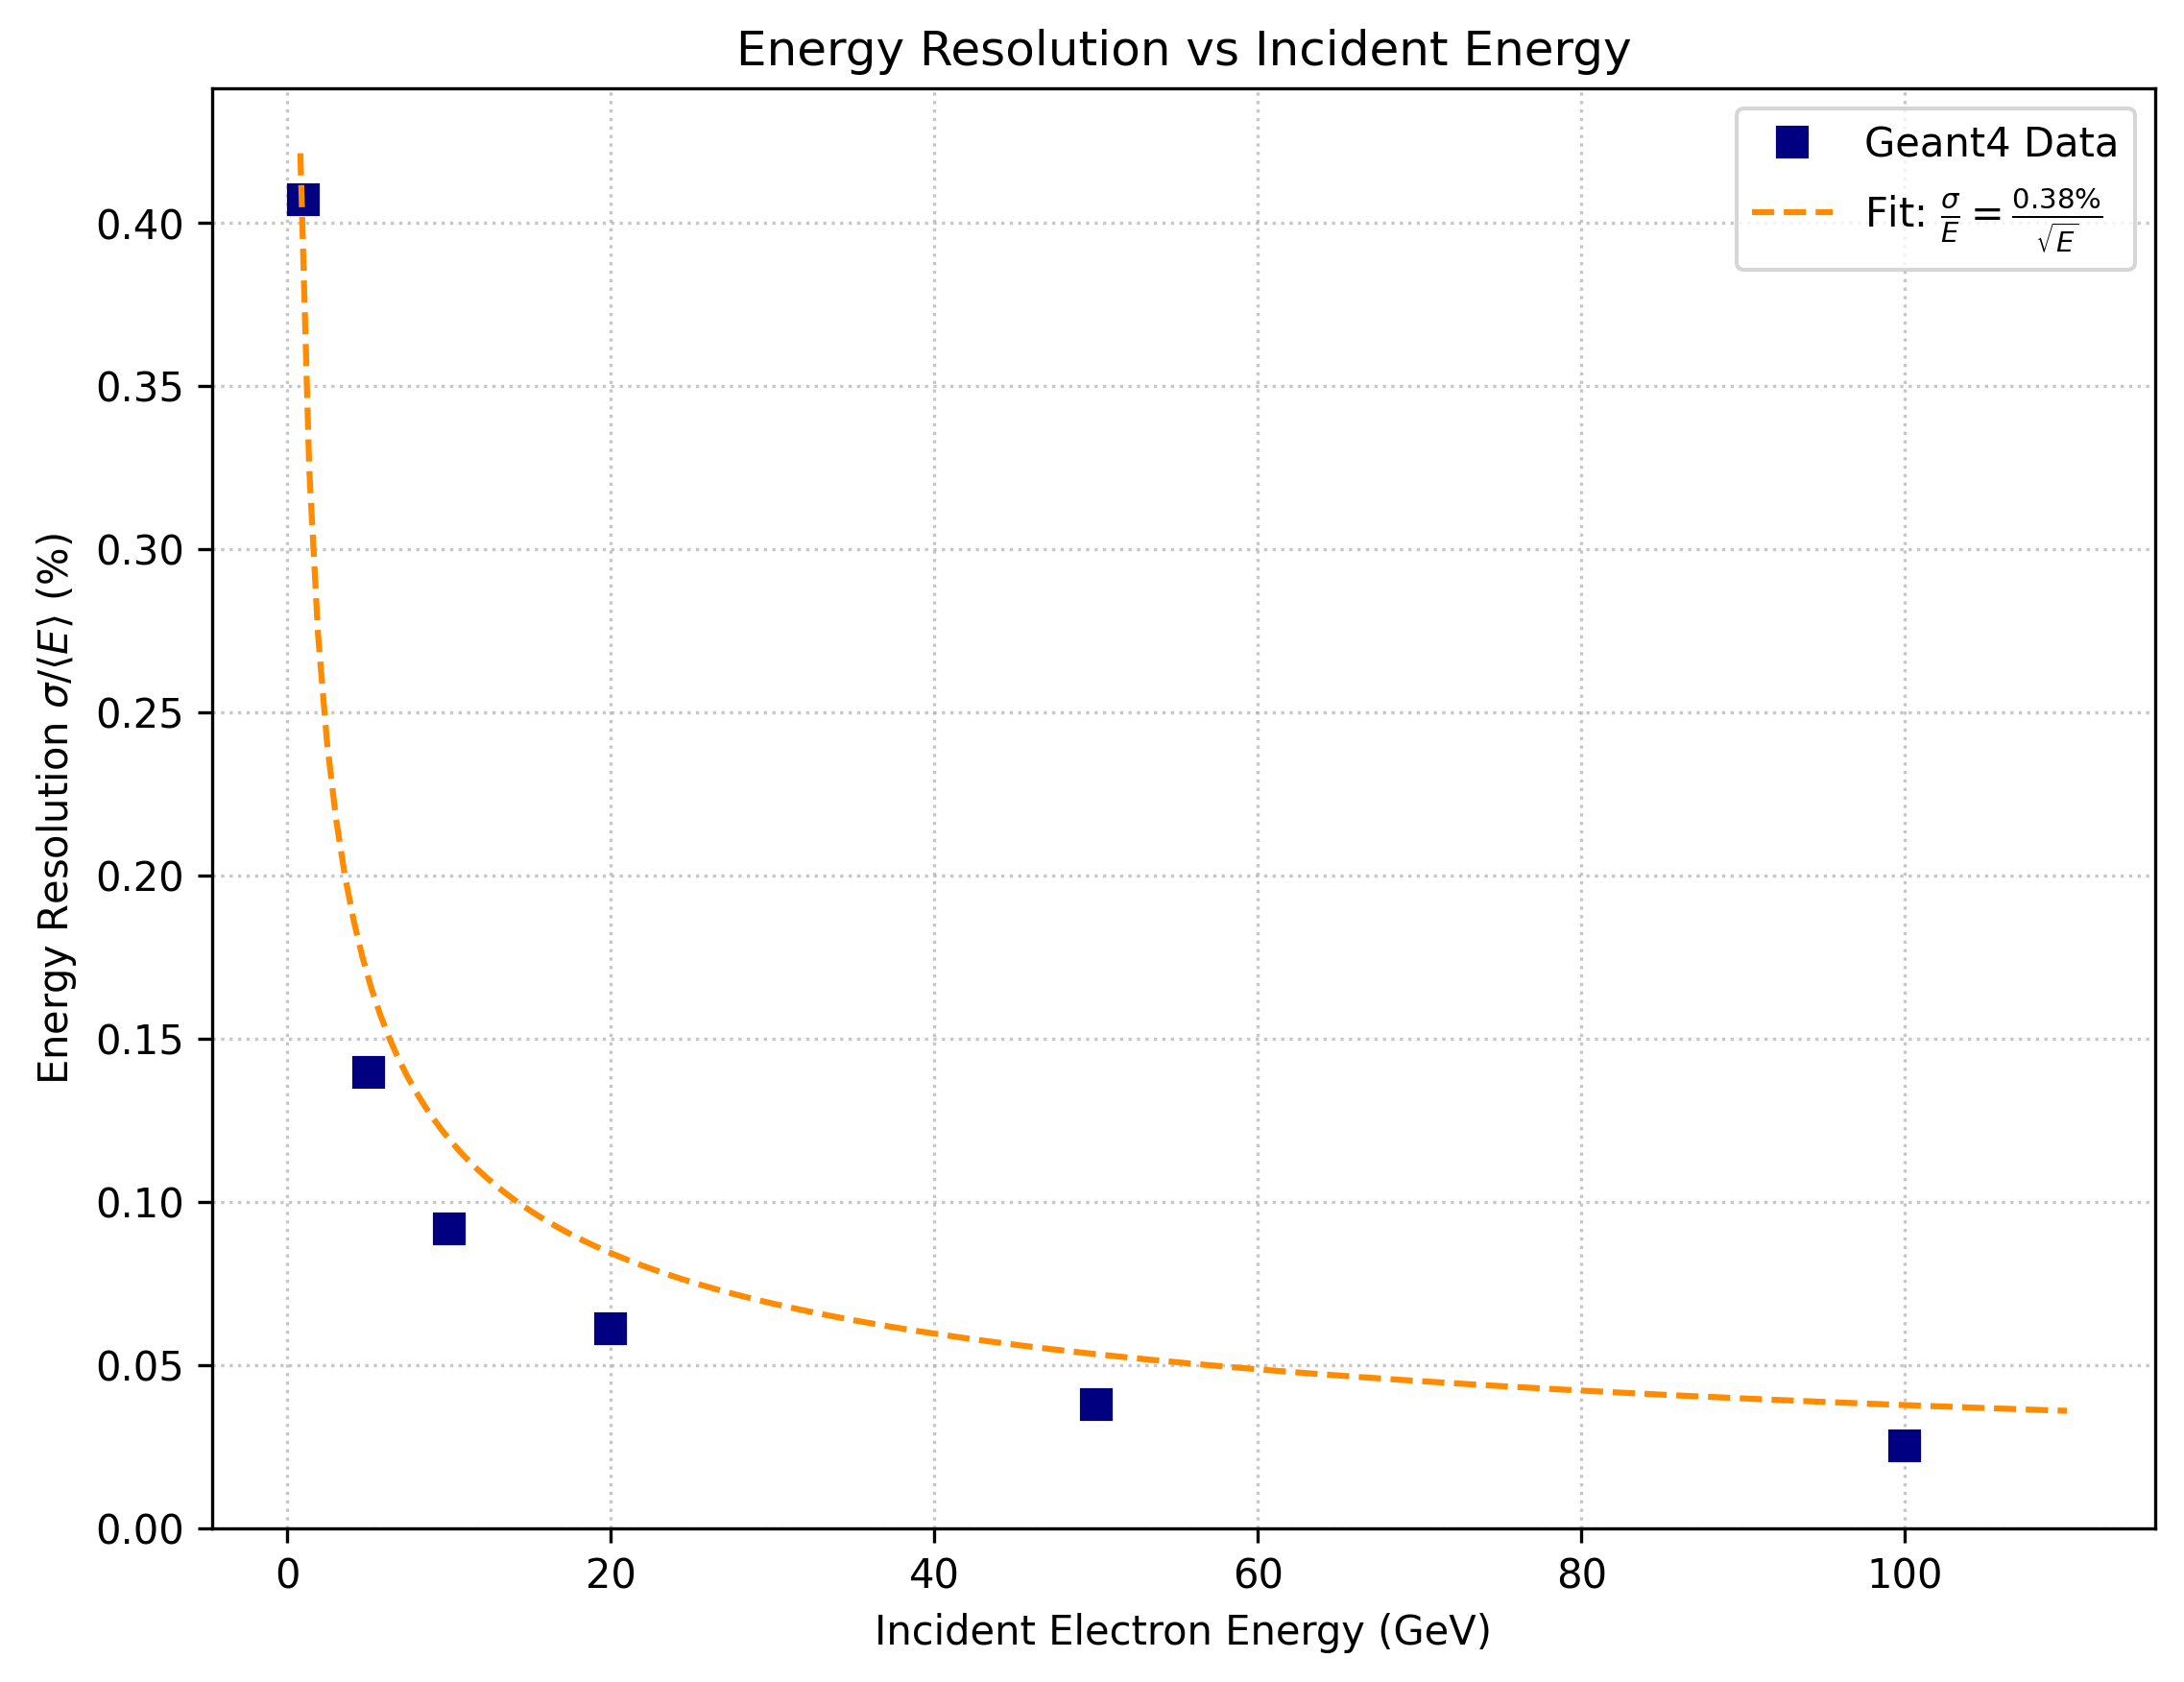
\includegraphics[width=0.39\textwidth]{Immagini/energy_response_analysis_1cm.png}
    \end{figure}

\end{frame}

\begin{frame}[noframenumbering]{Fluctuations in sampling calorimeters}
    
    \footnotesize % Riduce leggermente il font per far stare comodamente tutti i passaggi
    
    According to Rossi's Approximation B, the energy resolution is dominated by fluctuations in the number of charged particle crossings ($N_x$) in the active layers.
    
    \vspace{-0.1cm} % Recupera spazio sotto l'introduzione
    
    \begin{itemize}
        \setlength{\itemsep}{0pt} % Rimuove lo spazio verticale extra tra i punti elenco
        
        \item \textbf{Visible energy ($E_{vis}$):}
        \vspace{-0.2cm} % Annulla lo spazio bianco automatico dell'equazione
        \begin{equation*}
            E_{vis} = N_x \Delta E_{active} = N_x \left(\frac{dE}{dx}\right)_{active} d_{active}
        \end{equation*}
        
        \item \textbf{Number of crossings ($N_x$):} Expressed via the sampling fraction $f_{samp}$:
        \vspace{-0.2cm}
        \begin{equation*}
            f_{samp} = \frac{E_{vis}}{E} \implies N_x = \frac{f_{samp} E}{\Delta E_{active}}
        \end{equation*}
        
        \item \textbf{Poisson fluctuations:}
        \vspace{-0.2cm}
        \begin{equation*}
            \frac{\sigma(E_{vis})}{E_{vis}} = \frac{\sigma(N_x)}{N_x} = \frac{1}{\sqrt{N_x}} = \sqrt{\frac{\Delta E_{active}}{f_{samp} E}} \propto \sqrt{\frac{d_{active}}{f_{samp}}} \frac{1}{\sqrt{E}}
        \end{equation*}
    \end{itemize}
    
    At a fixed sampling fraction $f_{samp}$, the ratio of energy deposited in the active vs. passive layers is constant. Thus, the thicknesses are strictly proportional: $d_{active} \propto C \,d_{passive}$.
    
\end{frame}

\end{document}